\documentclass[a4paper,11pt,oneside]{report}

\usepackage[MScProject,lablogo]{EPFLreport}
\usepackage{xspace}
\usepackage[dvipsnames]{xcolor}
\usepackage{tcolorbox}
\usepackage{caption}
\usepackage{subcaption}


\title{Speeding up the InterPlanetary FileSystem (IPFS)}
\author{Guillaume Michel\\Computer Science -- Cybersecurity Master Student}
\supervisor{Cristina Basescu}
\adviser{Prof. Bryan Ford}


\setcounter{tocdepth}{2}
\newcommand{\sysname}{FooSystem\xspace}

\begin{document}
\maketitle

\maketoc

%%%%%%%%%%%%%%%%%%%%%%
\chapter{Introduction}
%%%%%%%%%%%%%%%%%%%%%%

Distributed data stores are widely used for different purposes and require in most cases strong responsiveness and partition resistance. Geo-replication is a solution for providing locality and decreasing interaction latency, in which data replicas are stored \textit{close} to the users interacting with it. The \textit{close} metric is a distance defined in term of ping latency, or the Round Trip Time (\textit{RTT}) between two peers.
The protocol Crux \cite{crux} developed by the DEDIS lab at EPFL enhances existing data stores with efficient locality techniques. It aims to provide low interaction latency, resilience to network partition, while keeping a low storage overhead. Crux has proven to be efficient on these aspects, when implemented and evaluated on top of two popular data stores: \textit{Redis} \cite{redis} an eventually consistent system, and \textit{CockroachDB} \cite{cockroachdb} a strongly consistent system.

The Inter Planetary File System (IPFS) is a peer-to-peer hypermedia protocol for storing data in a distributed file system. It aims to provide a unique file system that could host users' data in a big cloud hosted by the users themselves. The end goal of this system, as its name indicates, is to provide an optimized file system with geo-location based data replication, for inter planetary deployments.

IPFS, still under development, is one of the most advanced distributed file systems, thus we decided to implement Crux protocol on top of it and compare the performance of Vanilla IPFS versus Cruxified IPFS. IPFS vanilla for now, does not have a proper data orchestration between nodes to handle data replication, including files allocation to remote peers and replicas synchronization. We are going to use the software \textit{IPFS Cluster} to orchestrate data between IPFS daemons, for both experiments, in order to compare their performance.

IPFS is content addressed and combines ideas from \textit{Kademlia}, \textit{BitTorrent} and \textit{Git}. Locality is already enhanced by Kademlia \cite{kademlia} and Coral DSHT \cite{coral}. The goal of this project is to apply Crux protocol on IPFS, and to determine if it constitutes a major interaction latency improvement to IPFS.

%%%%%%%%%%%%%%%%%%%%
\chapter{Background}
%%%%%%%%%%%%%%%%%%%%

\section{Crux}

Crux \cite{crux} proposes an improvement to distributed systems such as data stores using locality features.
A complete reading of the paper is recommended for a better understanding of this project. Nonetheless, important notions for this project will be briefly discussed below.

Crux uses \textit{Available Responsive Areas} (ARAs) to preserve locality, defined as availability and responsiveness of user interactions. In this project, we will focus only on Crux responsiveness optimization. An ARA is a set of nodes located in a given latency diameter, i.e. the RTT between any two nodes of an ARA is upper bounded by the ARA latency diameter.
ARAs have at least one member, can overlap each other and are organized hierarchically by levels. The total number of level, $K$, is a parameter given to Crux, $K=3$ is the default value. Each node in the system is assigned a random level between $0$ and $K-1$. Each node is the \textit{root} of one or more ARAs,  of increasing network diameter. The root of an ARA is the node at its center. The higher level a node is assigned, the larger latency diameter its ARAs will be, and thus it will be the root of more ARAs. An ARA of level $K-1$ is a global ARA containing all nodes of the system, there can be multiple $K-1$ level ARAs. These ARAs provide an upper bound to interaction latency between any pair of nodes in the distributed system, this bound is a small multiple of the RTT between those two nodes.

In a cruxified system, an ARA is a set of connected nodes operating exactly as the underlying system would operate. For example, in our case, the underlying system being IPFS Cluster, an ARA would be an independent \textit{cluster} of IPFS Cluster instances. A cruxified system offers the same consistency guarantees as those offered by the underlying system.
Performing a write operation from a node $n$ in a cruxified system, is equivalent to performing a write operation in each ARA in which $n$ belongs. A replication factor can be specified for a write operation, as it would be in the underlying system. Performing a read operation is equivalent to performing a read operation in each ARA in which $n$ belongs, and returning the first response. Thus, the main idea described in Crux is data replication in strategic locations to decrease operation latency.

\section{IPFS}

IPFS \cite{ipfs}, designed and built by \textit{Protocol Labs} \cite{protocollabs}, is a complex system under development, with documentation scattered on multiple websites, the most complete being the official documentation website \cite{docipfs}. Due to ongoing work, some parts of the system are not properly documented yet and some features are incomplete. A few IPFS key features will be discussed in this section.

Nodes running IPFS are identified by a NodeID which is the cryptographic hash of a public-key, created with S/Kademlia’s static crypto puzzle \cite{skad}, in \texttt{multihash} format. Multihash \cite{multihash} is a protocol for creating hash digests, where multiple hash functions can coexist. The format is the following: \texttt{<hash-func-type><digest-length><digest-value>}. Here is an example:

\begin{tcolorbox}
\texttt{122041dd7b6443542e75701aa98a0c235951a28a0d851b11564d20022ab11d2589a8} \\
\-\ \-\ \-\ \-\ Hashing function: \texttt{sha2-256} (code in hex: \texttt{0x12})\\
\-\ \-\ \-\ \-\ Length: 32 (in hex: \texttt{0x20})\\
\-\ \-\ \-\ \-\ Digest: \texttt{41dd7b6443542e75701aa98a0c235951a28a0d851b11564d20022ab11d2589a8}
\end{tcolorbox}

Nodes store their public and private key pair locally. A node can also be identified by the \textit{multiaddress} on which it is running IPFS. Multiaddress \cite{multiaddr} is a format for encoding addresses defined by Protocol Labs. Here is an example of an IPFS node multiaddress:

\texttt{/ip4/104.236.76.40/tcp/4001}

Objects are identified by a Content IDentifier or CID \cite{cid}, based on the content’s cryptographic hash. This implies that files are identified by their content. There are currently two version of CIDs developped by \textit{Protocol Labs}: CIDv0 and CIDv1. IPFS is currently moving from CIDv0 to CIDv1. CIDv0 uses base 58-encoded multihashes starting with \texttt{Qm}, while CIDv1 is more flexible and is composed of 1) a multibase prefix, specifying the encoding used for the remainder of the CID 2) a CID version identifier, which indicates its version of CID (\texttt{0x01}), 3) a multicodec identifier, indicating the format of the target content 4) the corresponding multihash. Here are examples of both versions:

\texttt{CIDv0}: \texttt{QmfDWkL9K1bEutSYd8wod8se7Z8AQnUav7EU1UKabBbYhk}\\
\-\ \-\ \-\ \-\ \-\ \-\ \-\ \texttt{CIDv1}: \texttt{zb2rhe5P4gXftAwvA4eXQ5HJwsER2owDyS9sKaQRRVQPn93bA}


\subsection{Routing}

IPFS uses a Distributed Sloppy Hash Table (DSHT) defined by M. Freedman and D. Mazière in Coral \cite{coral}, augmented with concepts from S/Kadmelia \cite{skad}. A few concepts from Kademlia \cite{kademlia}, S/Kadmelia
and Coral used in IPFS implementation are discussed below.

Kademlia \cite{kademlia} is a Distributed Hash Table (DHT) with 160-bit keys, inspired by Chord \cite{chord} in which the \textit{XOR distance} is used as a metric of distance between hashes. XOR distance between two hashes $h1$ and $h2$ is computed as $\delta(h1,h2)=h1 \oplus h2$. Furthermore, like Chord's clockwise circle metric, \textit{XOR} is unidirectional. Each node keeps a list of $k$ ($k=20$ by default) node addresses and IDs for nodes at a distance between $2^i$ and $2^{i+1}$ from itself for $0 \leq i < 160$, thus forming 160 buckets of $k$-nodes. Buckets do not need to be full. Whenever a node receives a message from a peer, it adds it to the corresponding bucket, if it is not already full. Those buckets implement a least-recently seen eviction policy, except that nodes answering to periodic ping requests are never removed from the list.
During a node or key lookup, the lookup initiator first selects $\alpha$ nodes ($\alpha=3$ by default) from the closest bucket to the target ID. It is going to send \texttt{FIND\_NODE(ID)} RPC to those $\alpha$ nodes, that will reply with their closest known node's NodeID and address to the target ID. The lookup initiator will repeat this procedure iteratively with the newly received nodes until it reaches its target. S/Kademlia \cite{skad} improves the security of Kademlia mostly by generating secure NodeIDs and signing exchanged messages. Each node creates and stores a PKI key pair. The key creation includes a proof-of-work crypto puzzle to make Sybils generation expensive. The NodeID is the cryptographic hash of the node's public key, and the node signs the messages it sends with its private key.

M. Freedman and D. Mazière \cite{coral} claim that \textit{DHTs provide the wrong abstraction} as a node responsible for a very popular file can quickly become overloaded. They also claim that \textit{DHTs have poor locality} as most of DHTs implementation are not location aware. They introduce a new abstraction called DSHT, standing for Distributed Sloppy Hash Table. DSHTs support both frequent fetches and store of the same hash table key sacrificing the consistency of DHTs. In a DSHT, data can be stored on any nodes, and its locations are stored in the hash table.
A DSHT provides the same interface as a DHT, except that a \textit{key} can have multiple \textit{values}.

In Coral design, each node is member of several DSHTs, of increasing network diameter, defined as the maximum RTT between any two nodes in the DSHT. DSHT are organized in layers, and allow a hierarchical lookup. Each node has the same identifier in all DSHTs it belongs, allowing it to reduce the storage overhead. When writing data, the data is stored in all DSHTs in which the writer belongs. When reading data, all DSHTs in which the reader belongs are queried, and the search ends at the first hit. When data is cached somewhere in a Coral DSHT, any member of the DSHT can locate a copy without having to query farther away than the DSHT diameter. Ideas developed in Coral are in a way similar to those developed in Crux.

The implementation of the DHT used by IPFS is called \textit{libp2p Kademlia DHT} \cite{libp2p}. The implementation is largely based on Kademlia, with 256-bit keys, augmented with notions from S/Kademlia and Coral. It uses the XOR distance metric as defined in Kademlia. The data structure backing this system is a k-bucket routing table, inspired from Kademlia. The default bucket value is $k=20$, and there are at most 256 buckets, which is the size of a SHA265 hash. The concurrency of node and value lookup is limited by the parameter $\alpha$, with $\alpha=3$ by default, implying no more than 3 inflight requests at any given time. DHT's keys are CIDs. When looking up an entry in the DHT, the implementor should wait for at least $Q$ (quorum) responses from distinct nodes as a consistency guarantee before returning an answer. When looking up for a key $K$, the search is performed iteratively from the local store until the implementor gets $Q$ responses.

Small values, equal or less than 1KB, are stored directly on the DHT. For larger values, the DHT stores the NodeIDs of peers that can serve the block.

\subsection{Block Exchange}

Block Exchange is done through the BitSwap Protocol \cite{bitswap}, also developed by Protocol Labs. The BitSwap protocol is a generalization of BitTorrent’s data exchange protocol \cite{bittorrent} working with arbitrary DAGs. It uses BitTorrent's quasi tit-for-tat strategy that rewards nodes who contribute to each other, and punishes nodes who only leech others’ resources. As in BitTorrent, IPFS peers track the availability of file pieces, prioritizing sending rarest blocks first. This takes load off seeds, making non-seed peers capable of trading with each other.

\subsection{Objects and Files}

IPFS data structure is a generalization of the Git data structure. IPFS builds a Merkle DAG, a Directed Acyclic Graph where links between objects are cryptographic hashes of the targets embedded in the sources. Merkle DAG allows IPFS to achieve the following properties:
1) Content addressing: all content, including links is uniquely identified by \texttt{multihash} checksums, 2) Tamper resistance: IPFS is able to detect tampered content by verifying content's checksums and 3) Deduplication: objects that hold the same content are stored only once, to avoid duplication common portions of data.

IPFS objects can be traversed with a string path API. Paths work as they do in traditional UNIX filesystems. The Merkle DAG links make traversing the path easy. The path format is the following: \texttt{/ipfs/<hash-of-object>/<name-path-to-object>}. The \texttt{/ipfs} prefix allows mounting into existing systems at a standard mount point without conflict.

For now, path traversal causes multiple DHT lookups and is time consuming. For example, an object \texttt{foo/bar/baz.txt} location is resolved iteratively from its root. If \texttt{foo/} is stored at \texttt{ipfs/QmSjR3oJvJfVLL9LGLbDiG3dtcTRcUvhNrsggkUcTXv7Sy} then \texttt{baz.txt} will be located at \texttt{ipfs/QmSjR3oJvJfVLL9LGLbDiG3dtcTRcUvhNrsggkUcTXv7Sy/bar/baz.txt}. The \texttt{bar} and \texttt{baz.txt} also need to be resolved, thus causing 3 lookups for a single query. Protocol Labs is working on a new protocol \textit{graphsync} \cite{graphsync}, allowing peers to request a known sub-graph directly.

An object can be \textit{pinned} to ensure its survival. This ensures that the object will persist in a node's local storage upon failure or machine reboot. An object can be pinned \textit{locally} without being \textit{published}, and thus will be only locally accessible. A pinned object can be \textit{published} to be distributed globally, simply by adding its key to the DHT. All objects that are \textit{added} to IPFS are automatically pinned and published. Encrypted objects can be pinned and published as any other object.

IPFS also defines a set of objects for modeling a versioned filesystem on top of the Merkle DAG. This object model is similar to Git’s, and is made of: 1) \texttt{IPFS blocks} or \texttt{blobs}, 2) \texttt{lists}, 3) \texttt{trees} and 4) \texttt{commits}. The blob object contains an addressable unit of data, and represents a file. The list object represents a large or deduplicated file made up of several IPFS blobs concatenated together. The tree object in IPFS is similar to Git’s: it represents a directory, a map of names to hashes. The commit object in IPFS represents a snapshot in the version history of any object.

When reading a remote file, the IPFS peer first needs to query the DHT to get addresses of a provider of the root object of the file. It will then query the peers providing the file's objects based on their last answer latency. If the file is made of several, they will be downloaded concurrently.

\subsection{Naming}

As IPFS files are content addressed, they are immutable and thus a file identifier changes if a file gets modified. That is useful for the reasons mentioned before, but inconvenient to find the last version of a file. To address this issue, Protocol Labs developed the Inter Planetary Naming System (IPNS) \cite{ipns}, used to create and update mutable links to IPFS content. In IPNS, a \textit{name} is defined as the hash of a public key. The name is associated with a record containing information about the hash it links to, signed by the corresponding private key. To create a mutable file, one should publish a name, with the initial file, and when modifying it, one should specify the published name.

IPNS name: \texttt{/ipns/QmPD8QJKiVTh2TzYZg67twKLdPKrnh7QU98GBJe2hWcEoi}

DNSLink \cite{dnslink} is an alternative to IPNS offering more readable names. DNSLink uses DNS TXT records to map a human readable name to the last version of an IPFS object. This is an example of DNSLink mapping:

\noindent\texttt{/ipns/ipfs.io $\rightarrow$ /ipfs/bafybeiclyleqzl5f3irlg2jaxip7fjhp37d2lwm6cfwsgded7nkm3456ty}

Community members are currently exploring ways to use blockchains to store common name records.

\subsection{Implementations}

IPFS has currently two implementations: one in Golang (Go), and one in JavaScript (JS). It offers an HTTP API, as well as a client command line interface. It is possible to interact with the IPFS daemon via these interfaces, for example to \texttt{add}, \texttt{pin} or \texttt{get} a file, \texttt{resolve} ipfs names, \texttt{query} the DHT for values or peers etc. This project uses the \texttt{go-ipfs} \cite{go-ipfs} implementation, which is the most advanced one.

As seen in its specifications, IPFS has no file tracking feature. Thus, IPFS offers no consistency model, and is not able to handle file replication tasks, namely replicas allocation and synchronization.

\section{IPFS Cluster}
IPFS Cluster \cite{ipfs-cluster} provides data orchestration for a set of connected IPFS daemons. IPFS Cluster handles data allocation, replication, and synchronization across a \textit{cluster} of peers, as IPFS does not provide it. It does so by tracking a global \textit{pinset}, that is replicated on all the peers in the cluster. This global pinset, basically keeps track of all data updates, i.e. for each file, which peer is storing it, the file's replication factor, the last update. The pinset thus needs to be consistent on all peers.

IPFS Cluster is a program running on top of IPFS and interacting with the IPFS daemon through the IPFS API port. In order to create a cluster between multiple IPFS instances, it is necessary to run one IPFS Cluster daemon for each IPFS daemon. It is possible to run multiple IPFS Cluster instances on top of the same IPFS instance. It is still under heavy development, thus some features are not totally optimized and may change in the coming years.

IPFS Cluster has two main programs, \texttt{ipfs-cluster-service} and \texttt{ipfs-cluster-ctl} defined in the \texttt{ipfs-cluster} repository \cite{ipfs-cluster-repo}. The first one is the IPFS Cluster daemon that initializes the cluster instance and runs it. The second one is a Command Line Interface client to interact with IPFS Cluster daemon, i.e. adding files, listing pins etc. It is also possible to use the restAPI to interact with \texttt{ipfs-cluster-service}.

A cluster can be created by any IPFS Cluster daemon, and upon creation, a random 32-byte hex-encoded \texttt{secret} is generated and acts as a shared key, required to join the cluster.
Any IPFS Cluster daemon can join a cluster on startup if it knows the \texttt{secret} value and the \texttt{multiaddress} of a peer already in the cluster. Each cluster is given parameters such as a global minimum and maximum replication factor, a list of trusted peers, the consensus component etc.\cite{cluster-config}.

When pinning a file to a cluster, it is possible to choose a specific replication factor for this file, and/or the peers allocations. If no allocation is specified by the client, the cluster will allocate the file according to a priority list, based on the free IPFS repository space. The developers plan to provide a greater allocation flexibility in the future. As IPFS objects are immutable, they are not supposed to be modified. For convenience, IPFS Cluster allows files updates, if a the \texttt{update} option is set and initial CID specified while pinning update with the IPFS Cluster client. The file allocation will not change, and files will be updated at the nodes storing them. IPNS was certainly used to implement this feature, but it is currently not documented.

IPFS Cluster allows writing a file to cluster, but not reading from a cluster. The write operation makes sure that the file is pinned accordingly to the allocation policy in the cluster. The IPFS Cluster instance communicates files to allocate and pinset information to the IPFS instance. The write operation returns, once a consensus between cluster peers is made on the update. Thus it is possible that when the write operation returns, the file is not pinned yet to remote locations. The read operation has to be done by the IPFS instance, and thus is not cluster specific. 
If an IPFS daemon is member of multiple clusters (and thus has multiple IPFS Cluster instances running on top of its API), performing a read operation will trigger requests to all connected peers, regardless of their cluster membership.

IPFS Cluster is currently implemented with two different consensus component options: Raft and CRDT. The consensus component must be chosen when initializing IPFS Cluster. Raft is the default consensus component of IPFS Cluster.

\subsection{Raft}

Raft \cite{raft} is a consensus algorithm similar to Paxos \cite{paxos}, and is used in other databases such as CockroachDB \cite{cockroachdb}.

The progress of an update to the pinset works as follow. First, at cluster startup, the peers elect a leader that has to get a majority of votes. Once a leader is elected, all write operation have to go through the leader. (1) The block to be written is concurrently transferred to all nodes assigned to store it, (2) then the update is sent by the client to the leader, (3) the leader broadcasts the update to all peers, (4) peers acknowledge the received update to the leader (5), the leader waits for a majority of acknowledgments, and (6) it confirms the update to the client and broadcasts that the update was accepted to all peers. If the leader fails, a new leader is elected after a timeout. Thus, Raft guarantees strong consistency to the database it runs on.

IPFS Cluster's implementation of Raft is very faithful to the original algorithm, and thus guarantees strong consistency to the cluster. A write operation of a single block file done in the cluster is expected to take around $3\times RTT + \mathcal{O}(c)$, $RTT$ being the average RTT between any pair of nodes in the cluster, and $\mathcal{O}(c)$ being a non-negligible constant time required to perform local computations. 

\subsection{CRDT}

A CRDT, standing for \textit{Conflict-free Replicated Data Types}, is a data type whose operations commute when they are concurrent and was defined by Marc Shapiro et al. \cite{crdt}. CRDTs consistency model is \textit{Strong Eventual Consistency} (SEC) defined for the purpose of CRDT. Strong Eventual Consistency is an Eventual Consistency model, and a replicated object is defined as Strongly Eventually Consistent if it is Eventually Consistent and replicas that have delivered the same updates have equivalent state. CRDT operations must be commutative and idempotent. 

A simple example of CRDT is a distributed counter. The counter is initially set to $0$ at all replicas. Then nodes can \texttt{ADD(N)} to increase the counter by $N$ or \texttt{SUBSTITUTE(N)} to decrease the counter of $N$. The nodes having received the same updates will be in the same state, as addition is a commutative operation. The nodes will eventually receive all updates, the order in which they arrive is not important.

A SEC object does not satisfy sequential consistency. To illustrate this principle, let's to take a set $S$, initially empty, with two defined operations \texttt{ADD(e)} and \texttt{REMOVE(e)}, to add or remove an element to the set. In sequential execution, the last update wins, implying that after the sequence \texttt{ADD(e)} $\rightarrow$ \texttt{REMOVE(e)}, $e \notin S$. In SEC environments, commutative rules must be defined to decide which concurrent operation wins. For example, one can decide that \texttt{ADD(e)} always wins over \texttt{REMOVE(e)}. Thus both sequences of operations \texttt{ADD(e)} $\rightarrow$ \texttt{REMOVE(e)} and \texttt{REMOVE(e)} $\rightarrow$ \texttt{ADD(e)} imply $e \in S$, the order in which the updates are received does not matter. Different rules can be chosen, such as the update resulting in a neutral state in case of conflict, or the update with the lowest hash wins etc. Concurrent updates on distinct objects can be applied normally. 

\textit{Merkle-CRDTs} have been introduced by Héctor Sanjuán et al. \cite{merkle-crdts}, to build some distributed application on top of IPFS. Héctor Sanjuán is himself an IPFS Cluster developer. The operation of Merkle-CRDTs is out of the scope of this report, but an intuition of how they work will be given. To sum up the ideas exposed in this paper, events can be seen as nodes in a DAG, the \textit{last} event(s) being the root node(s). \textit{Merkle-Clock} ($\mathcal{M}(e)$) is a kind of logical clock defining event causality. 

For example, if events $e_\alpha$ and $e_\beta$ are roots of their distinct DAG. Then, happens an event $e_\gamma$, such that $\mathcal{M}(e_\gamma) > \mathcal{M}(e_\alpha)$ and $\mathcal{M}(e_\gamma) > \mathcal{M}(e_\beta)$. $e_\gamma$'s DAG children will be  $e_\alpha$ and $e_\beta$. If $e_\delta$ happen concurrently to $e_\gamma$, and is contradictory to $e_\gamma$, the conflict is resolved the same way as in CRDT, described above. Each \textit{event} can contain a payload that is the actual update to a data structure.

IPFS Cluster CRDT mode is still under development, and has not much documentation. It offers equivalent performance as Raft mode, when tested on a network of 20 nodes. However, it is supposed to scale better than Raft for larger networks.

%%%%%%%%%%%%%%%%%%%%%%%%
\chapter{Design \& Implementation}
%%%%%%%%%%%%%%%%%%%%%%%%

\section{Cruxifying IPFS}
As the goal of this experiment is to compare the performance Vanilla IPFS with the performance Cruxified IPFS, we first had to Cruxify IPFS. This required to generate \textit{Available Responsive Areas} (ARAs) and to make IPFS use them. In order to create these ARAs, we had to select a distance metric for locality. We chose the RTT or ping distance between two nodes as the distance metric, for the RTT is the metric of internet locality. We generated the ARAs as defined in Crux \cite{crux}.

\vspace{0.8cm}

\begin{figure}[ht!]
  \centering
  \captionsetup{width=.6\linewidth}
  \captionsetup{justification=centering}
  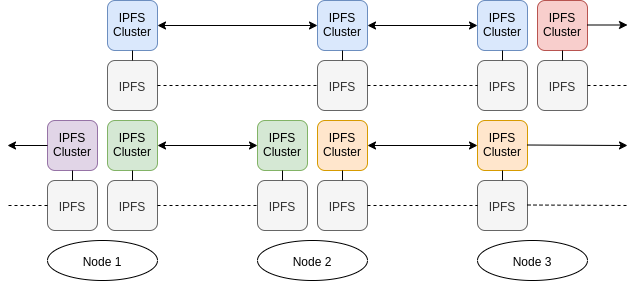
\includegraphics[width=.8\linewidth]{diagram.png}
  \caption{Structure of the IPFS and IPFS Cluster instances running on each node, in Cruxified IPFS.\\ Colors represent ARA membership.}
  \label{fig:diagram}
\end{figure}

As Crux should be applied on a system handling data replication, we needed to run IPFS Cluster on top of IPFS. There was two design possibilities: 1) running one IPFS instance per node, and multiple IPFS Cluster instances on top of each IPFS instance, or 2) running one IPFS instance per ARA in which the node belongs on each node, and one IPFS Cluster instance on top of each IPFS instance. We chose to use the second solution, depicted in Figure \ref{fig:diagram}, for it provides isolation between different IPFS instances, which is what is expected by Crux. As there is no read operation defined on a cluster, the read operation is performed on the IPFS instance directly. IPFS is not able to know in which cluster a remote node belongs to. Crux requires the ability of reading from a specific cluster, implying the incorrectness of the first solution. For example, node $n_0$ belongs to $ARA_0$ and $ARA_1$, and the closest replica of the file it wants to access to is stored at $n_1$ in $ARA_0$. Crux wants it to perform a read operation in both clusters, but IPFS is not aware of cluster existence, and will query twice the closest replica of the file at $n_1$. The first solution would, in most cases, perform the most optimized operation, thus returning the same performance as the second solution would return.

We had to choose a replication factor for IPFS Cluster, and wanted to select a realistic \textit{standard} replication factor even though there is no \textit{standard} replication factor as this system is not widely deployed. We estimated that three is a realistic replication factor, as data can still be available when two nodes fail, and a larger replication factor would not really make sense in ARAs of 20 nodes at most, the storage overhead would be too large. The minimum ARA size is defined by the replication factor, as it is impossible to allocate a file on three different nodes if the ARA don't contain a minimum of three nodes. Thus, the minimum ARA size is of three nodes.

Cruxified IPFS interface only includes the necessary features: a \texttt{WRITE(file)} command and a \texttt{READ(CID)} command. The \texttt{WRITE(file)} command writes a file concurrently to all ARAs in which the node belongs. The \texttt{READ(CID)} command tries concurrently to read a file, identified by its \texttt{CID} from all ARAs in which the node belongs, and returns the first response.

In a real world deployment, Cruxified IPFS interface would need to allow modifying existing files, which can be done through IPFS Cluster API. It would also need to synchronize modified files in non-global ARAs, which can be done by tracking files from its pinset in larger ARAs, and fetching updates from those. Both upgrade to the actual implementation should respect the consistency model of IPFS Cluster, which is Strong Consistency for Raft mode, and Eventual Consistency for CRDT mode.

The client design is kept simple and only includes necessary features. It allows users to perform writes and reads from a chosen node, and let smaller ARAs fetch updates from larger ARAs to achieve eventual consistency.

\section{Implementation}

All the code, its documentation and instructions on how to run and use it are available on Github, at \url{https://github.com/dedis/student_19_cruxIPFS}. A guide to configure and run an IPFS Cluster is also available on the repository. This section will cover implementation details such as the steps taken, the tools used and the challenges faced, but not how to run the code.

We mostly took inspiration from the DEDIS repositories \texttt{cothority\_template}\cite{cothority_template}, \texttt{CoSi} \cite{CoSi}, \texttt{paper\_crux} \cite{paper_crux} and 
\texttt{paper\_nyle} \cite{paper_nyle}. 
We started building the Cruxified IPFS implementation on top of the \texttt{cothority\_template} repository from the DEDIS lab, which is itself running on \texttt{Onet} \cite{onet}, also developed by DEDIS. The code was meant to be deployed on \texttt{Deterlab} \cite{deterlab}, and \texttt{cothority\_template} already handled the deployment using \texttt{Onet}.

\subsection{Onet}

The implementation uses \texttt{service} and \texttt{protocol} defined in the \texttt{Onet} package from the DEDIS lab. To cruxify IPFS and deploy it on the test beds.

We used a \textit{service} to compute the RTTs between any pair of nodes in the system, and build the ARAs for cruxified IPFS. The RTT computation was inspired from \texttt{paper\_nyle} repository. We detected a mistake and corrected the RTT computation algorithm used in \texttt{paper\_nyle}, for it was not getting symmetric results, which were needed to be able to create ARAs properly (i.e. \texttt{PING(\textit{n1},\textit{n2})}$\neq$\texttt{PING(\textit{n2},\textit{n1})}). The ARA creation process was also taken from \texttt{paper\_nyle}.

We used two \texttt{Onet} protocols to startup IPFS and IPFS Cluster instances. The first protocol is running from the root of the Onet tree, and broadcasts to all peers, signaling them to start their respective instances. They will iterate on all ARA trees in which the current node is the root, and start the second protocol on each one. The second protocol, nested in the first one, is run on each node and defines how to start the instances. It starts an IPFS instance and an IPFS Cluster instance running on top of it, for ARA where the current node is the root. Then it broadcasts to all the ARA's member to start their IPFS and IPFS Cluster with its own IPFS Cluster bootstrap address to join the ARA. Once this is done, they respond to the root of the ARA with the address they are using to run IPFS Cluster. The root of the ARA gathers all peer addresses. When the second protocol has run on all ARA trees in which the current node is the root, it will return all its different ARA peers addresses to the initiator of the first protocol. The initiator of the first protocol will then store these information on disk, which are used by the client to contact different IPFS Cluster instances running on different nodes.

\subsubsection{Bugs}

I discovered two bugs in \texttt{Onet}, and reported them to the developing team. It took a lot of time to spot that bugs were actually coming from \texttt{Onet} and not from the cruxified IPFS implementation, and to isolate the errors before reporting them. It took extra time that was obviously not planned beforehand, but I am happy to have helped improving \texttt{Onet}. I included the links to the Github associated pull requests for references.

Bug 1: \url{https://github.com/dedis/onet/pull/599}

Bug 2: \url{https://github.com/dedis/onet/pull/603}

\subsection{Client implementation}

To implement a client that can interact with this Cruxified IPFS and Vanilla IPFS, we used the default IPFS Cluster client defined in the \texttt{ipfs-cluster} \cite{ipfs-cluster-repo} repository. The client was using the information written on disk by the first protocol to contact nodes and make them perform operations.

\subsection{Deterlab deployement}

The implementation was deployed on Deterlab \cite{deterlab} because the platform allows us to define arbitrary network topologies that are more realistic than a local simulation. In order to create Deterlab experiments, we used scripts from the \texttt{paper\_crux} \cite{paper_crux} repository, slightly refactored for ease of use. \texttt{Onet} was very convenient in the deployment, as a local simulation can run remotely without having to change much code. It also offers functions to copy file to the remote servers, which was necessary to install IPFS and IPFS Cluster software. The \texttt{cothority} simulation prescript verifies that both programs are installed on the remote hosts, and handles installation in case they are not installed already.

As it was not convenient to get a clean output from the remote nodes (\texttt{ssh} to each nodes to recover output files), the simulation outputs a lot of logs to the console. Those logs can be caught by simple bash scripts running the simulation on the remote platform, getting all the logs, and parsing them to text files, used to plot graphs.

I experienced strange not easily reproducible issues with \texttt{Onet}, while connecting to a remote simulation. Onet was not able to \textit{find all children}, making the experiment impossible, until the topology get changed.

\section{Project limitations}

As the number of nodes one can book on Deterlab is quite limited, we were not able to perform performance tests with networks having more than 20 nodes. It would be interesting to test the same experiment on a network of a thousand nodes, but it is hard to find a such large network for rent.

Another project limitation is that the platform does not handle topologies with very large RTT between nodes (i.e $RTT >$ 10 sec). It would be interesting to run the experiment with a network in an inter planetary setting, to test and try to improve inter planetary deployment.

%%%%%%%%%%%%%%%%%%%%
\chapter{Evaluation}
%%%%%%%%%%%%%%%%%%%%

We evaluated multiple networks of IPFS nodes organized in clusters under different settings, in order to measure IPFS latency performances. In all experiments, we compared Vanilla IPFS to Cruxified IPFS as described in the Design \& Implementation chapter. The experiment taken to illustrate the results is the most representative and meaningful experiment conducted. Data related to other experience is not demonstrated, but will be shortly discussed.

The experiment consists in measuring interaction latencies in the network between pairs of nodes. Pairs of nodes are generated at random, the first node writes a file on IPFS Cluster, and once it is pinned the second node reads the file that was just written. The measured interaction latency is the sum of the Write latency and the Read latency in each pair of nodes.

The differences between the multiple conducted experiments are the following. We changed the number of hosts used to create the topology. The more hosts the topology contains, the more realistic the experiment will be, compared to a real world deployment. Unfortunately, we could not get more than 20 nodes because of the deployment platform's limitation. We made the RTT between the nodes vary, and all the results we got had a similar shape, a maximal RTT between two nodes of 400 ms, which is a meaningful range for earth deployment. We tried to write and read files of multiple sizes, some fitting in a single block, and some requiring multiple blocks, and got similar results in both cases.

The selected experiment was conducted on a quasi-random graph topology of 20 nodes, with random RTTs between two nodes up, going up to 400ms. The nodes are machines with 16GiB RAM, Xeon E5-2420 v2 processor, running under Ubuntu 14.04 connected through 100Mib/s interfaces. The selected file size is 2KiB, hence the file fits in a single IPFS block (a block being at most 256KiB). We used the Crux parameter $K=3$ levels of landmarks. The experience was conducted with IPFS Cluster both in Raft and CRDT modes. We generated a sequence of 2000 pairs of nodes randomly and measured Write and Read latency for each pair. We used the same sequence of pairs of nodes when comparing Cruxified with Vanilla IPFS, and Raft mode with CRDT mode.

\begin{figure}[htbp!]
\centering
\begin{subfigure}{.5\textwidth}
  \centering
  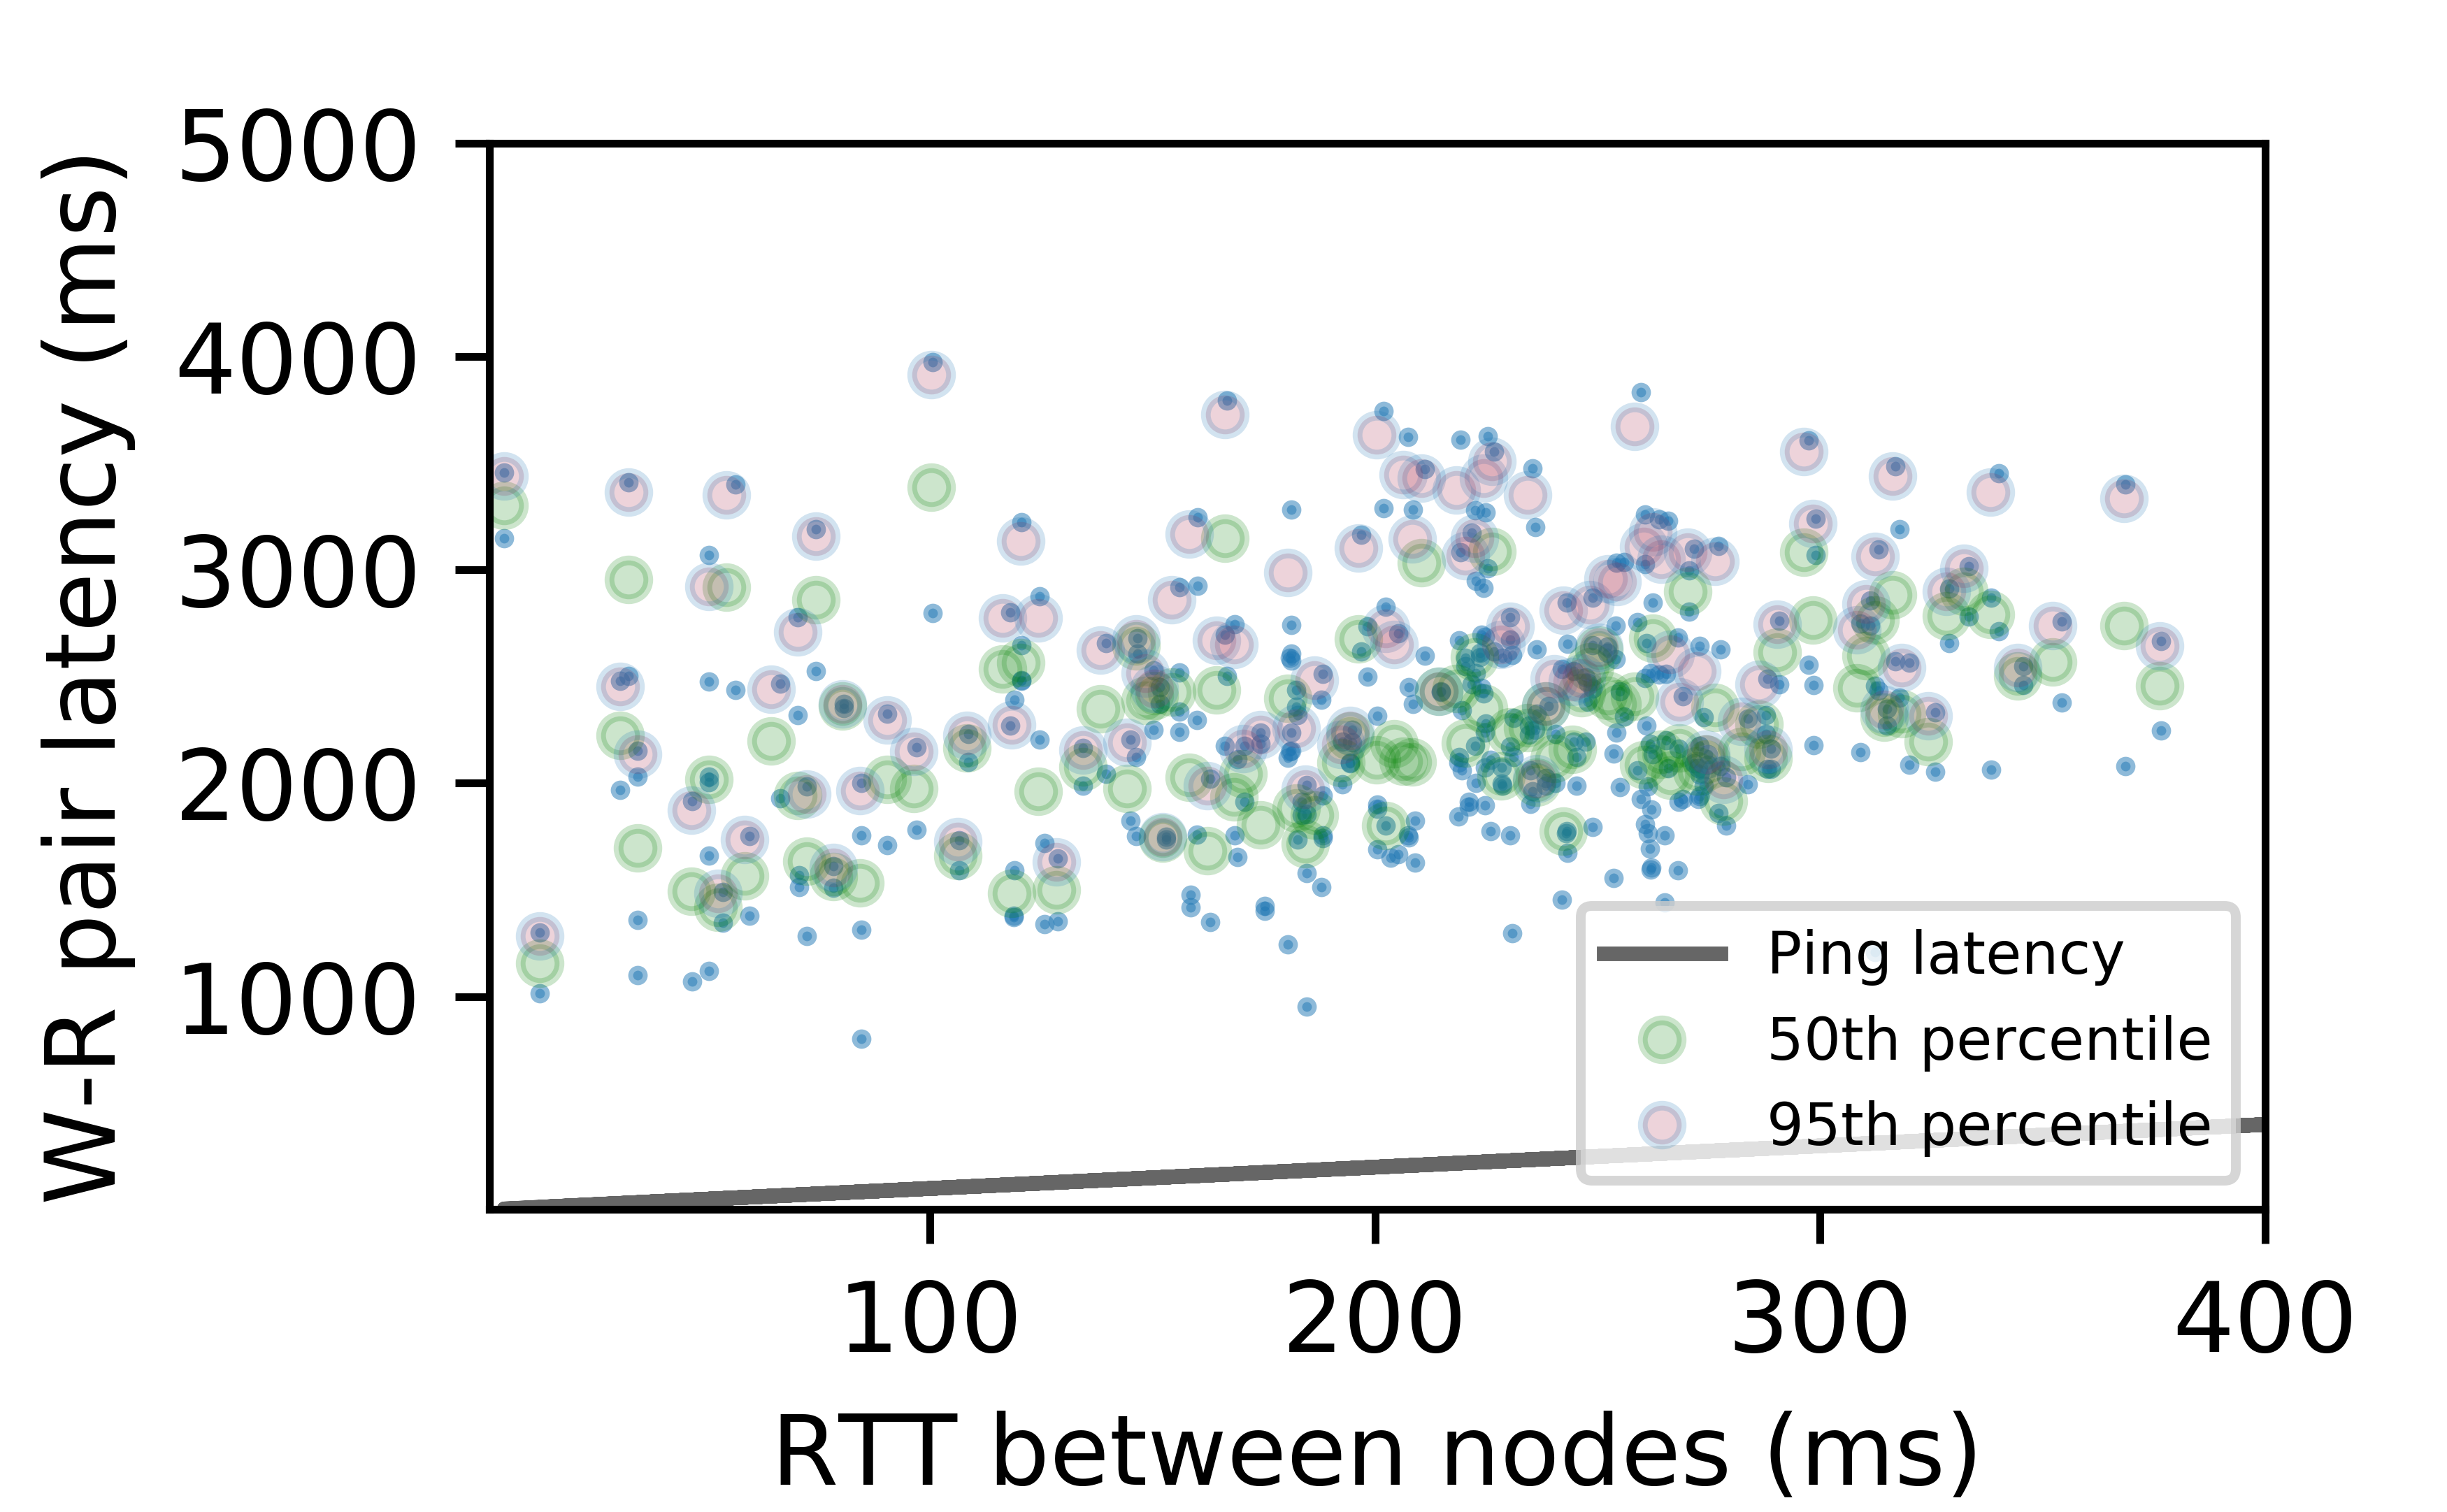
\includegraphics[width=1\linewidth]{graphs/plot_zoom_vanilla_raft.png}
  \caption{Vanilla IPFS}
  \label{fig:crdt1}
\end{subfigure}%
\begin{subfigure}{.5\textwidth}
  \centering
  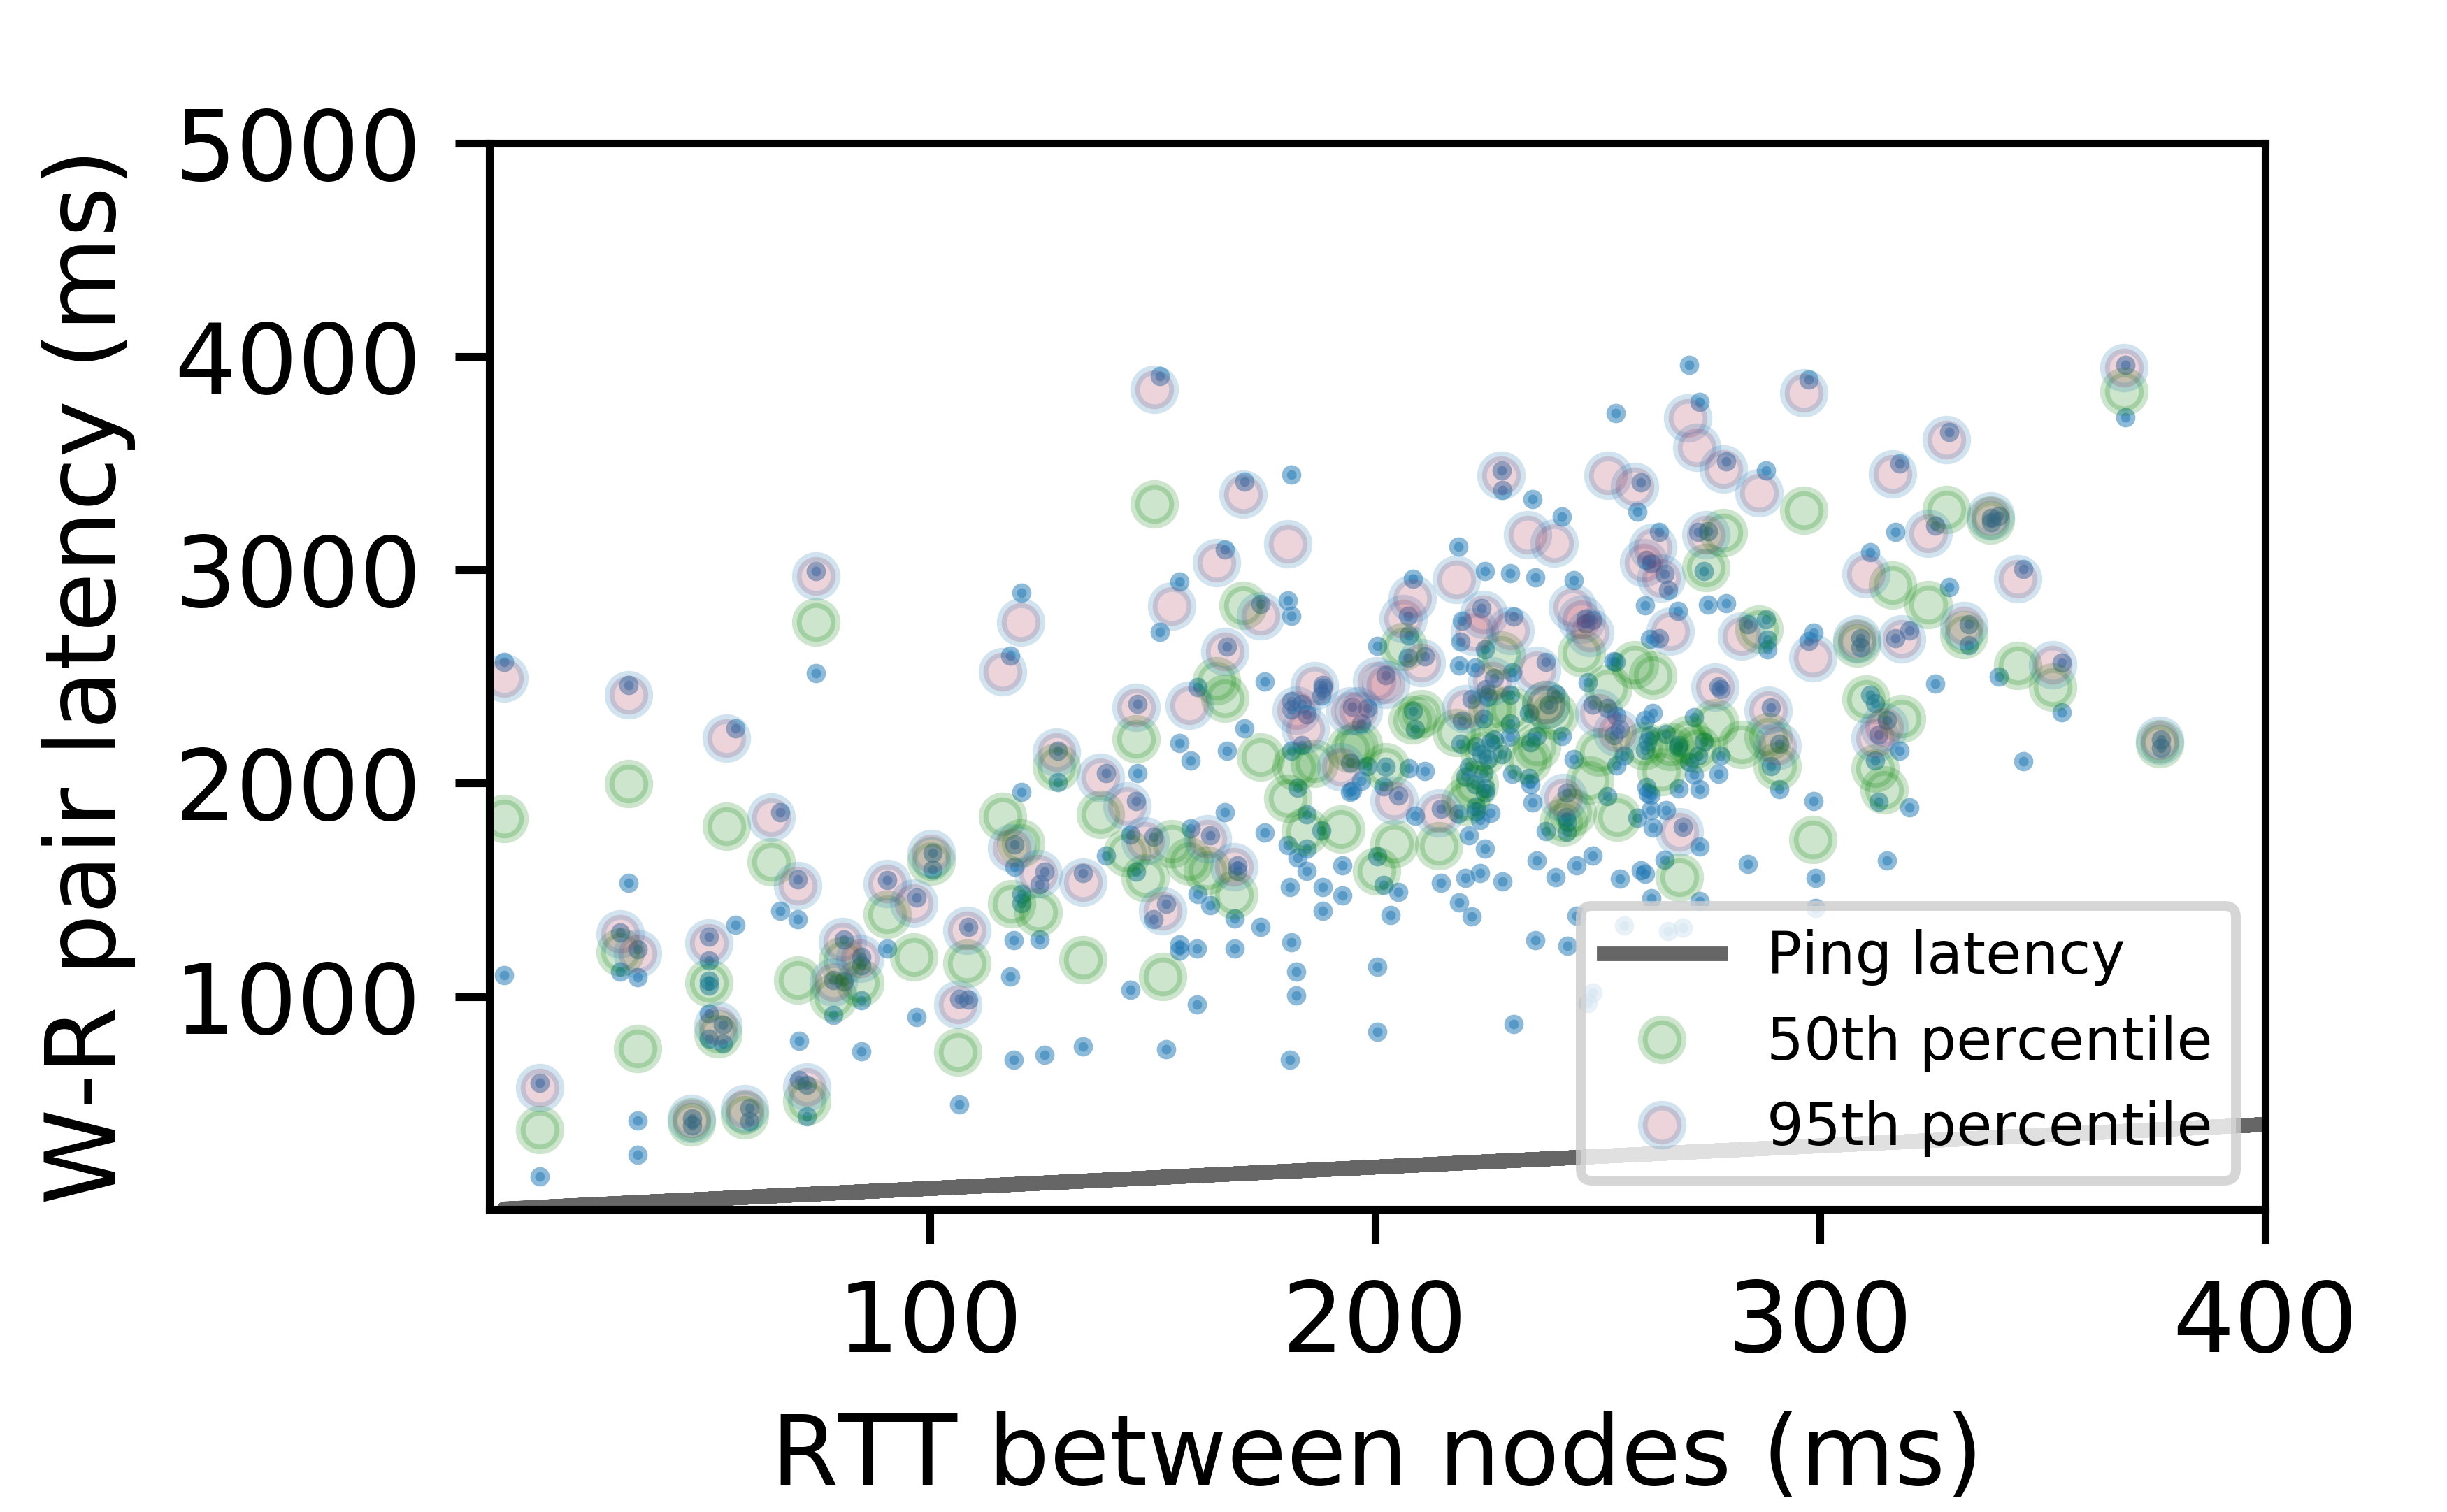
\includegraphics[width=1\linewidth]{graphs/plot_zoom_cruxified_raft.png}
  \caption{Cruxified IPFS}
  \label{fig:crdt2}
\end{subfigure}
\caption{CRDT mode, Write+Read pair latency}
\label{fig:crdt}
\end{figure}

\begin{figure}[htbp!]
\centering
\begin{subfigure}{.5\textwidth}
  \centering
  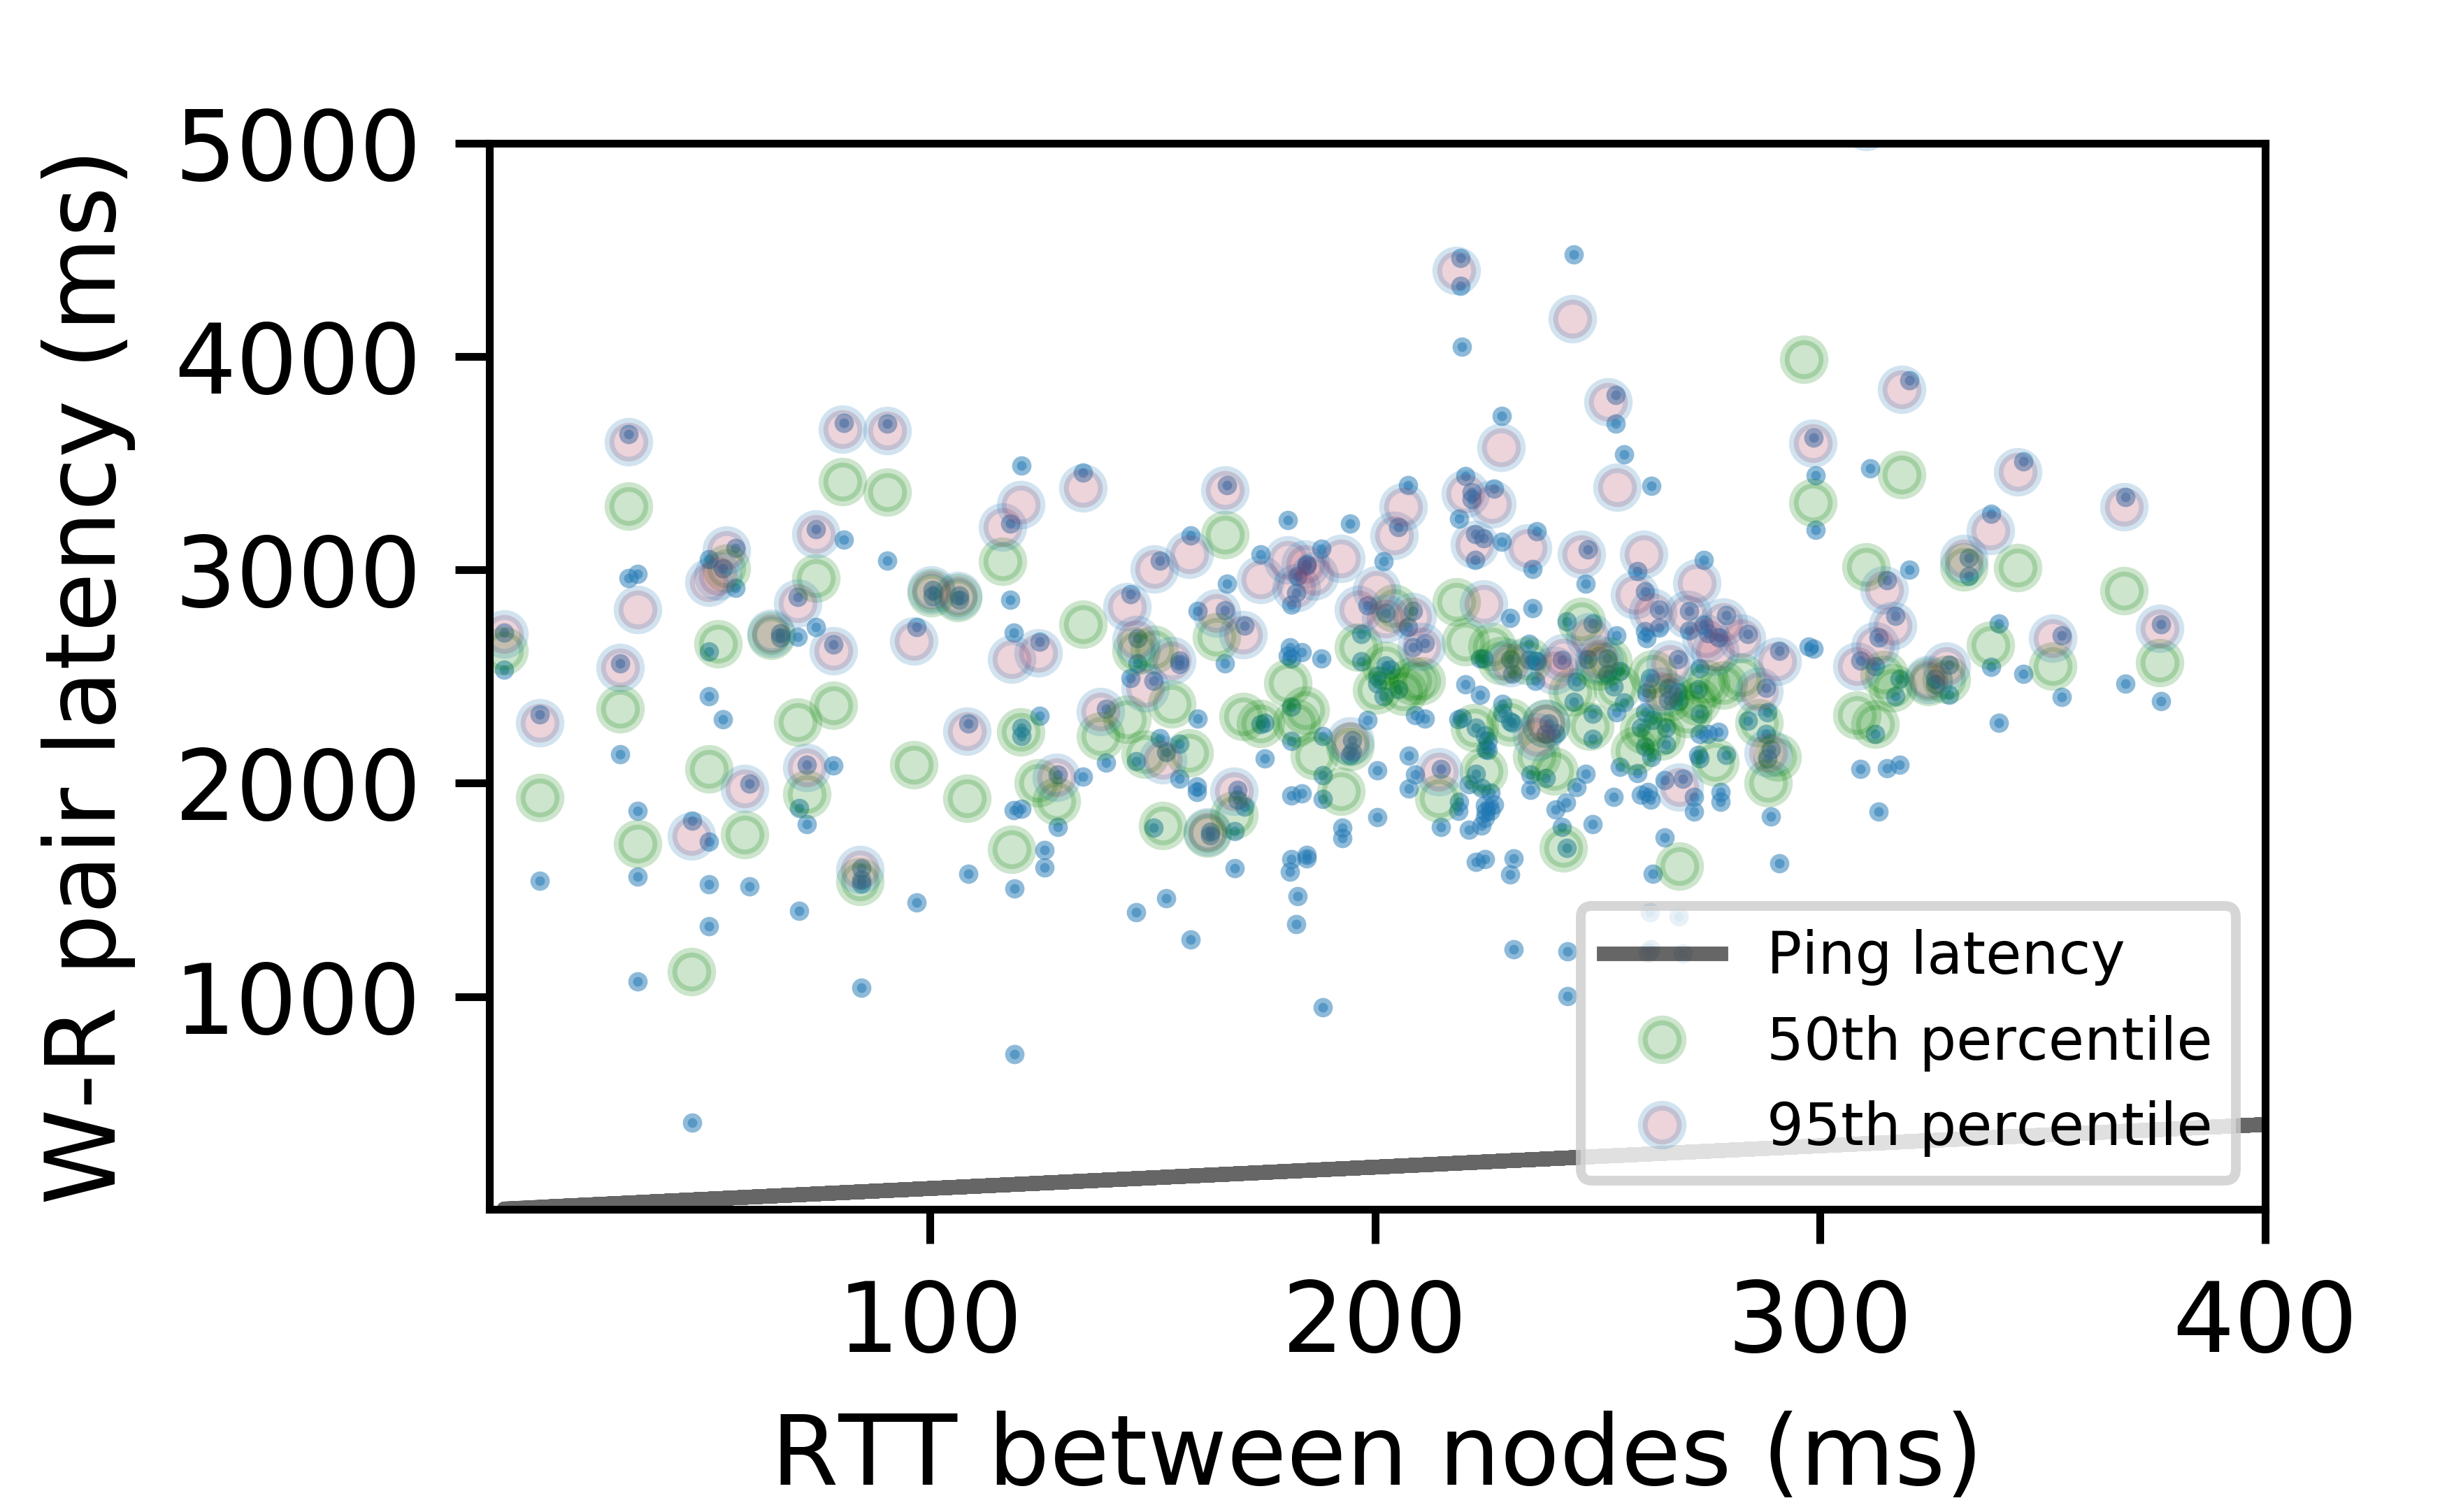
\includegraphics[width=1\linewidth]{graphs/plot_zoom_vanilla_crdt.png}
  \caption{Vanilla IPFS}
  \label{fig:zoom1}
\end{subfigure}%
\begin{subfigure}{.5\textwidth}
  \centering
  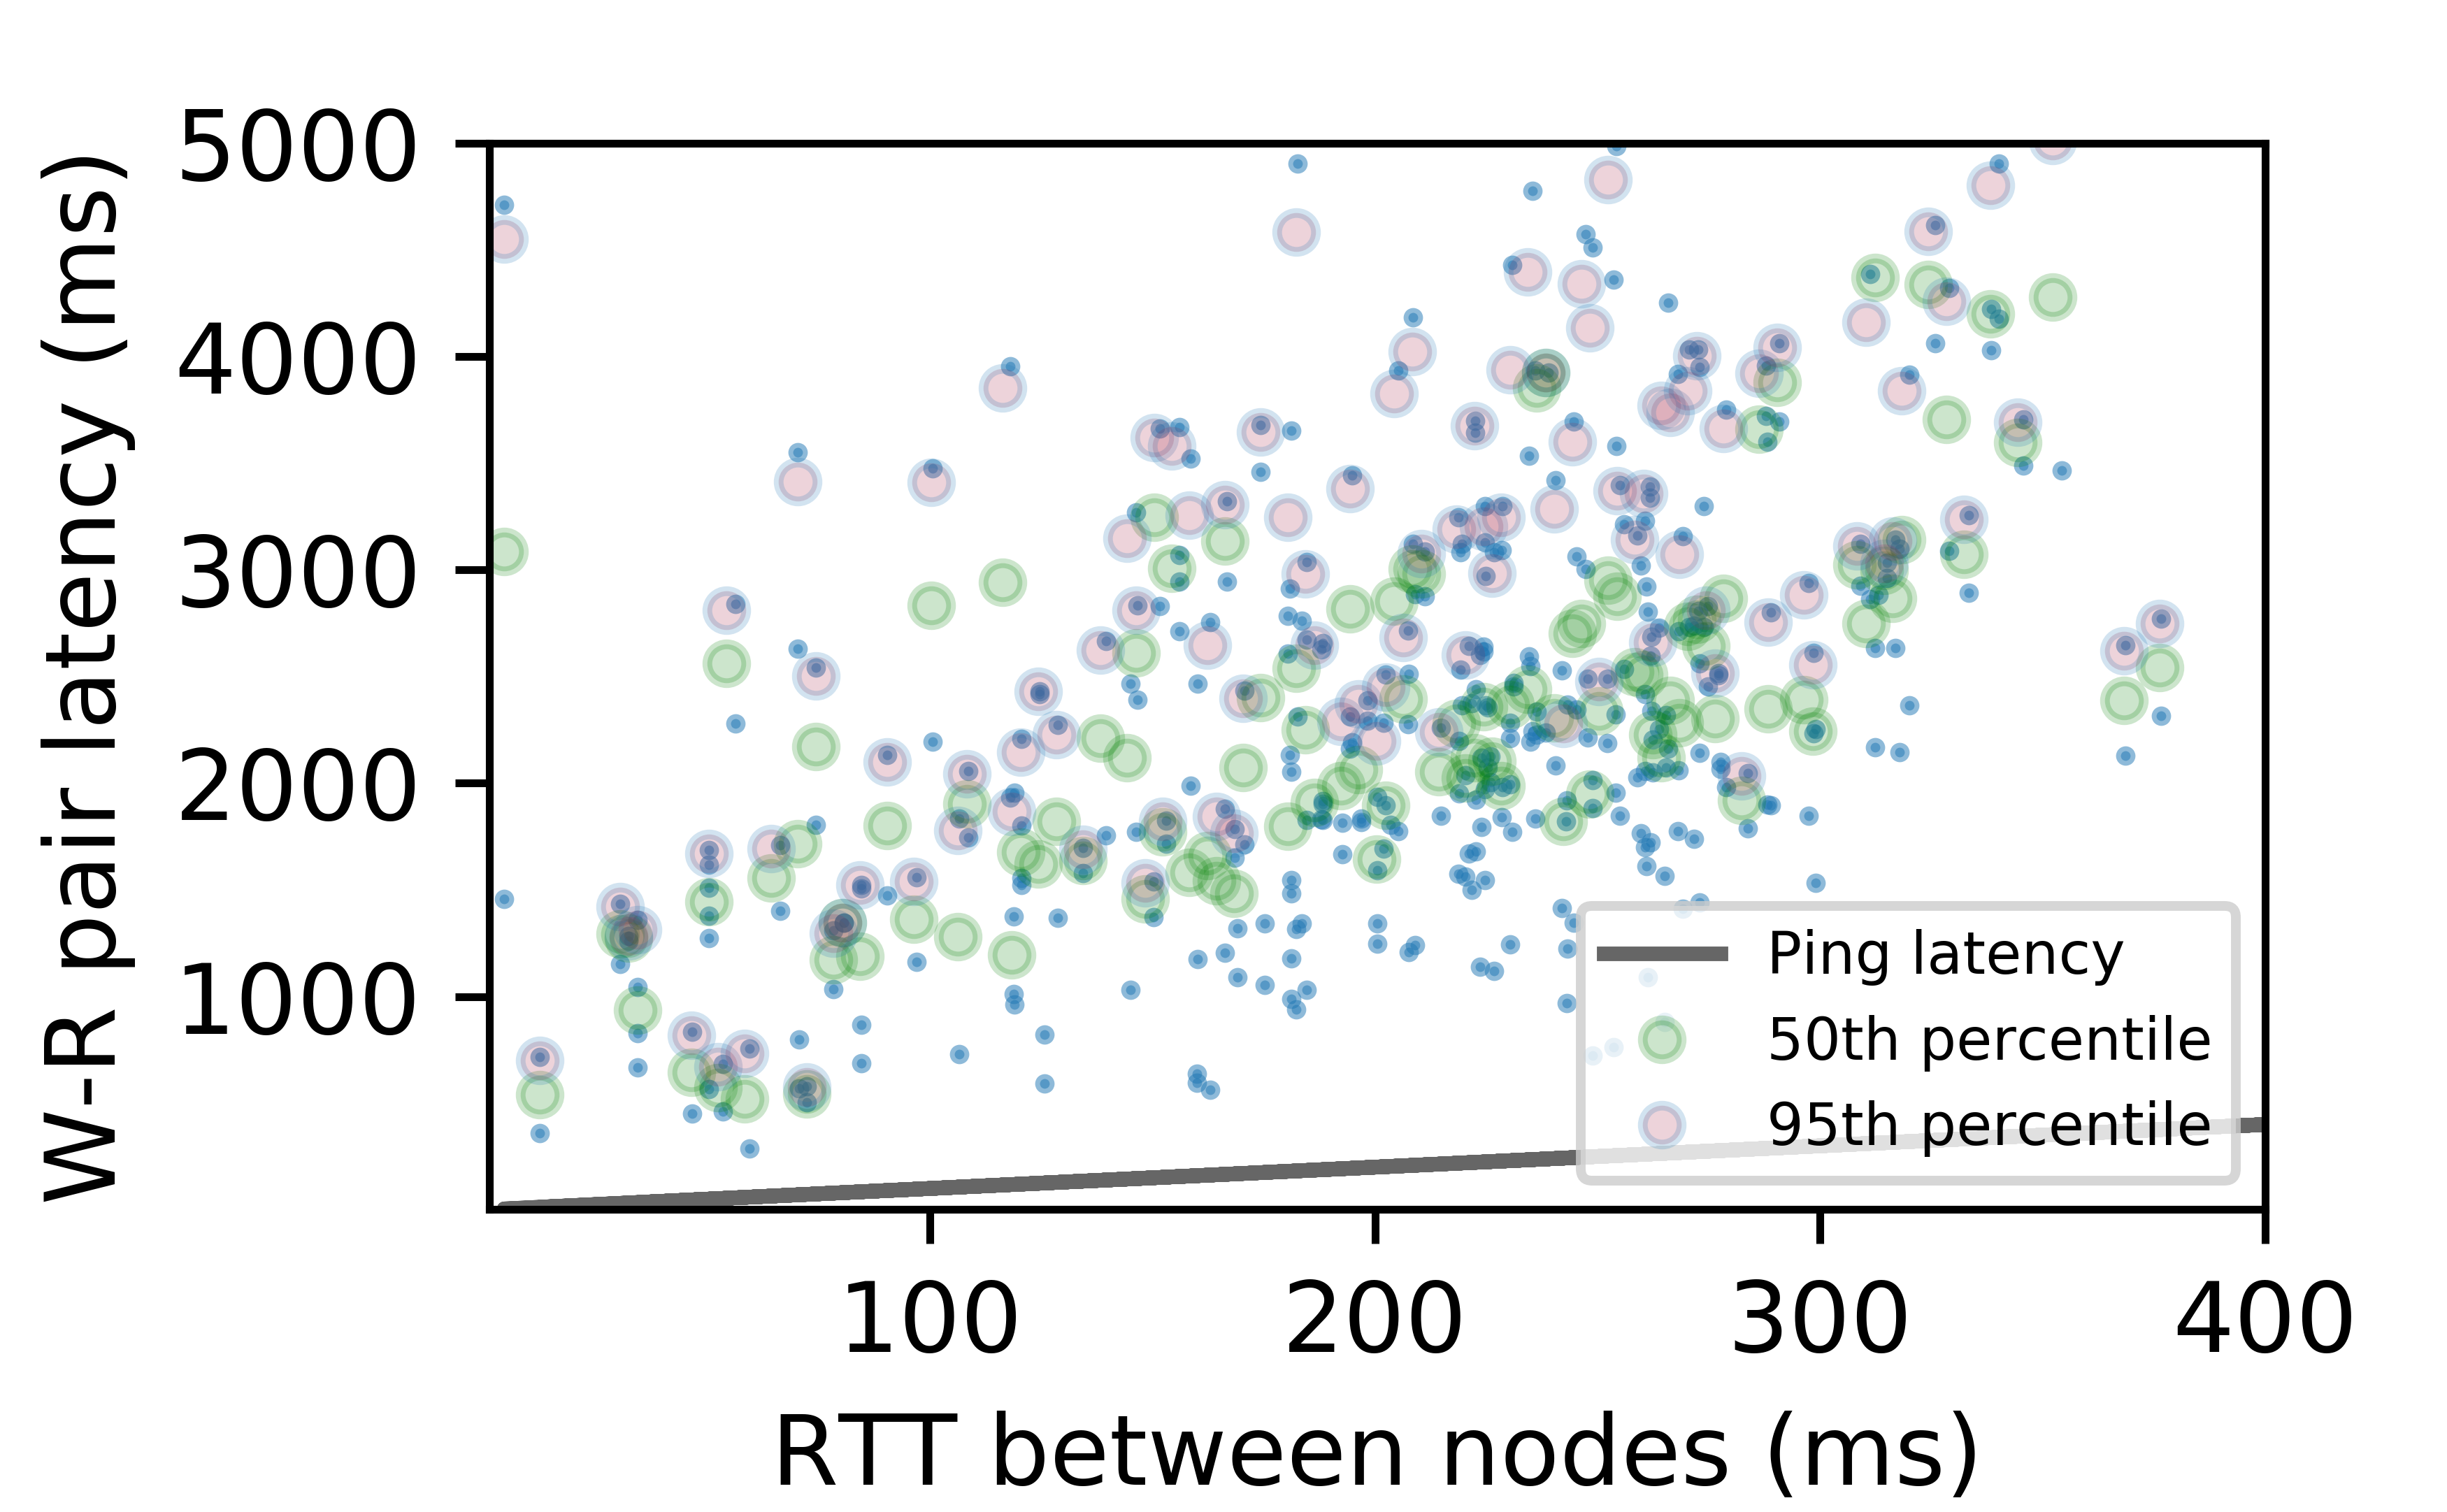
\includegraphics[width=1\linewidth]{graphs/plot_zoom_cruxified_crdt.png}
  \caption{Cruxified IPFS}
  \label{fig:zoom2}
\end{subfigure}
\caption{Raft mode, Write+Read pair latency}
\label{fig:zoom}
\end{figure}

\begin{figure}[h!]
\centering
\begin{subfigure}{.5\textwidth}
  \centering
  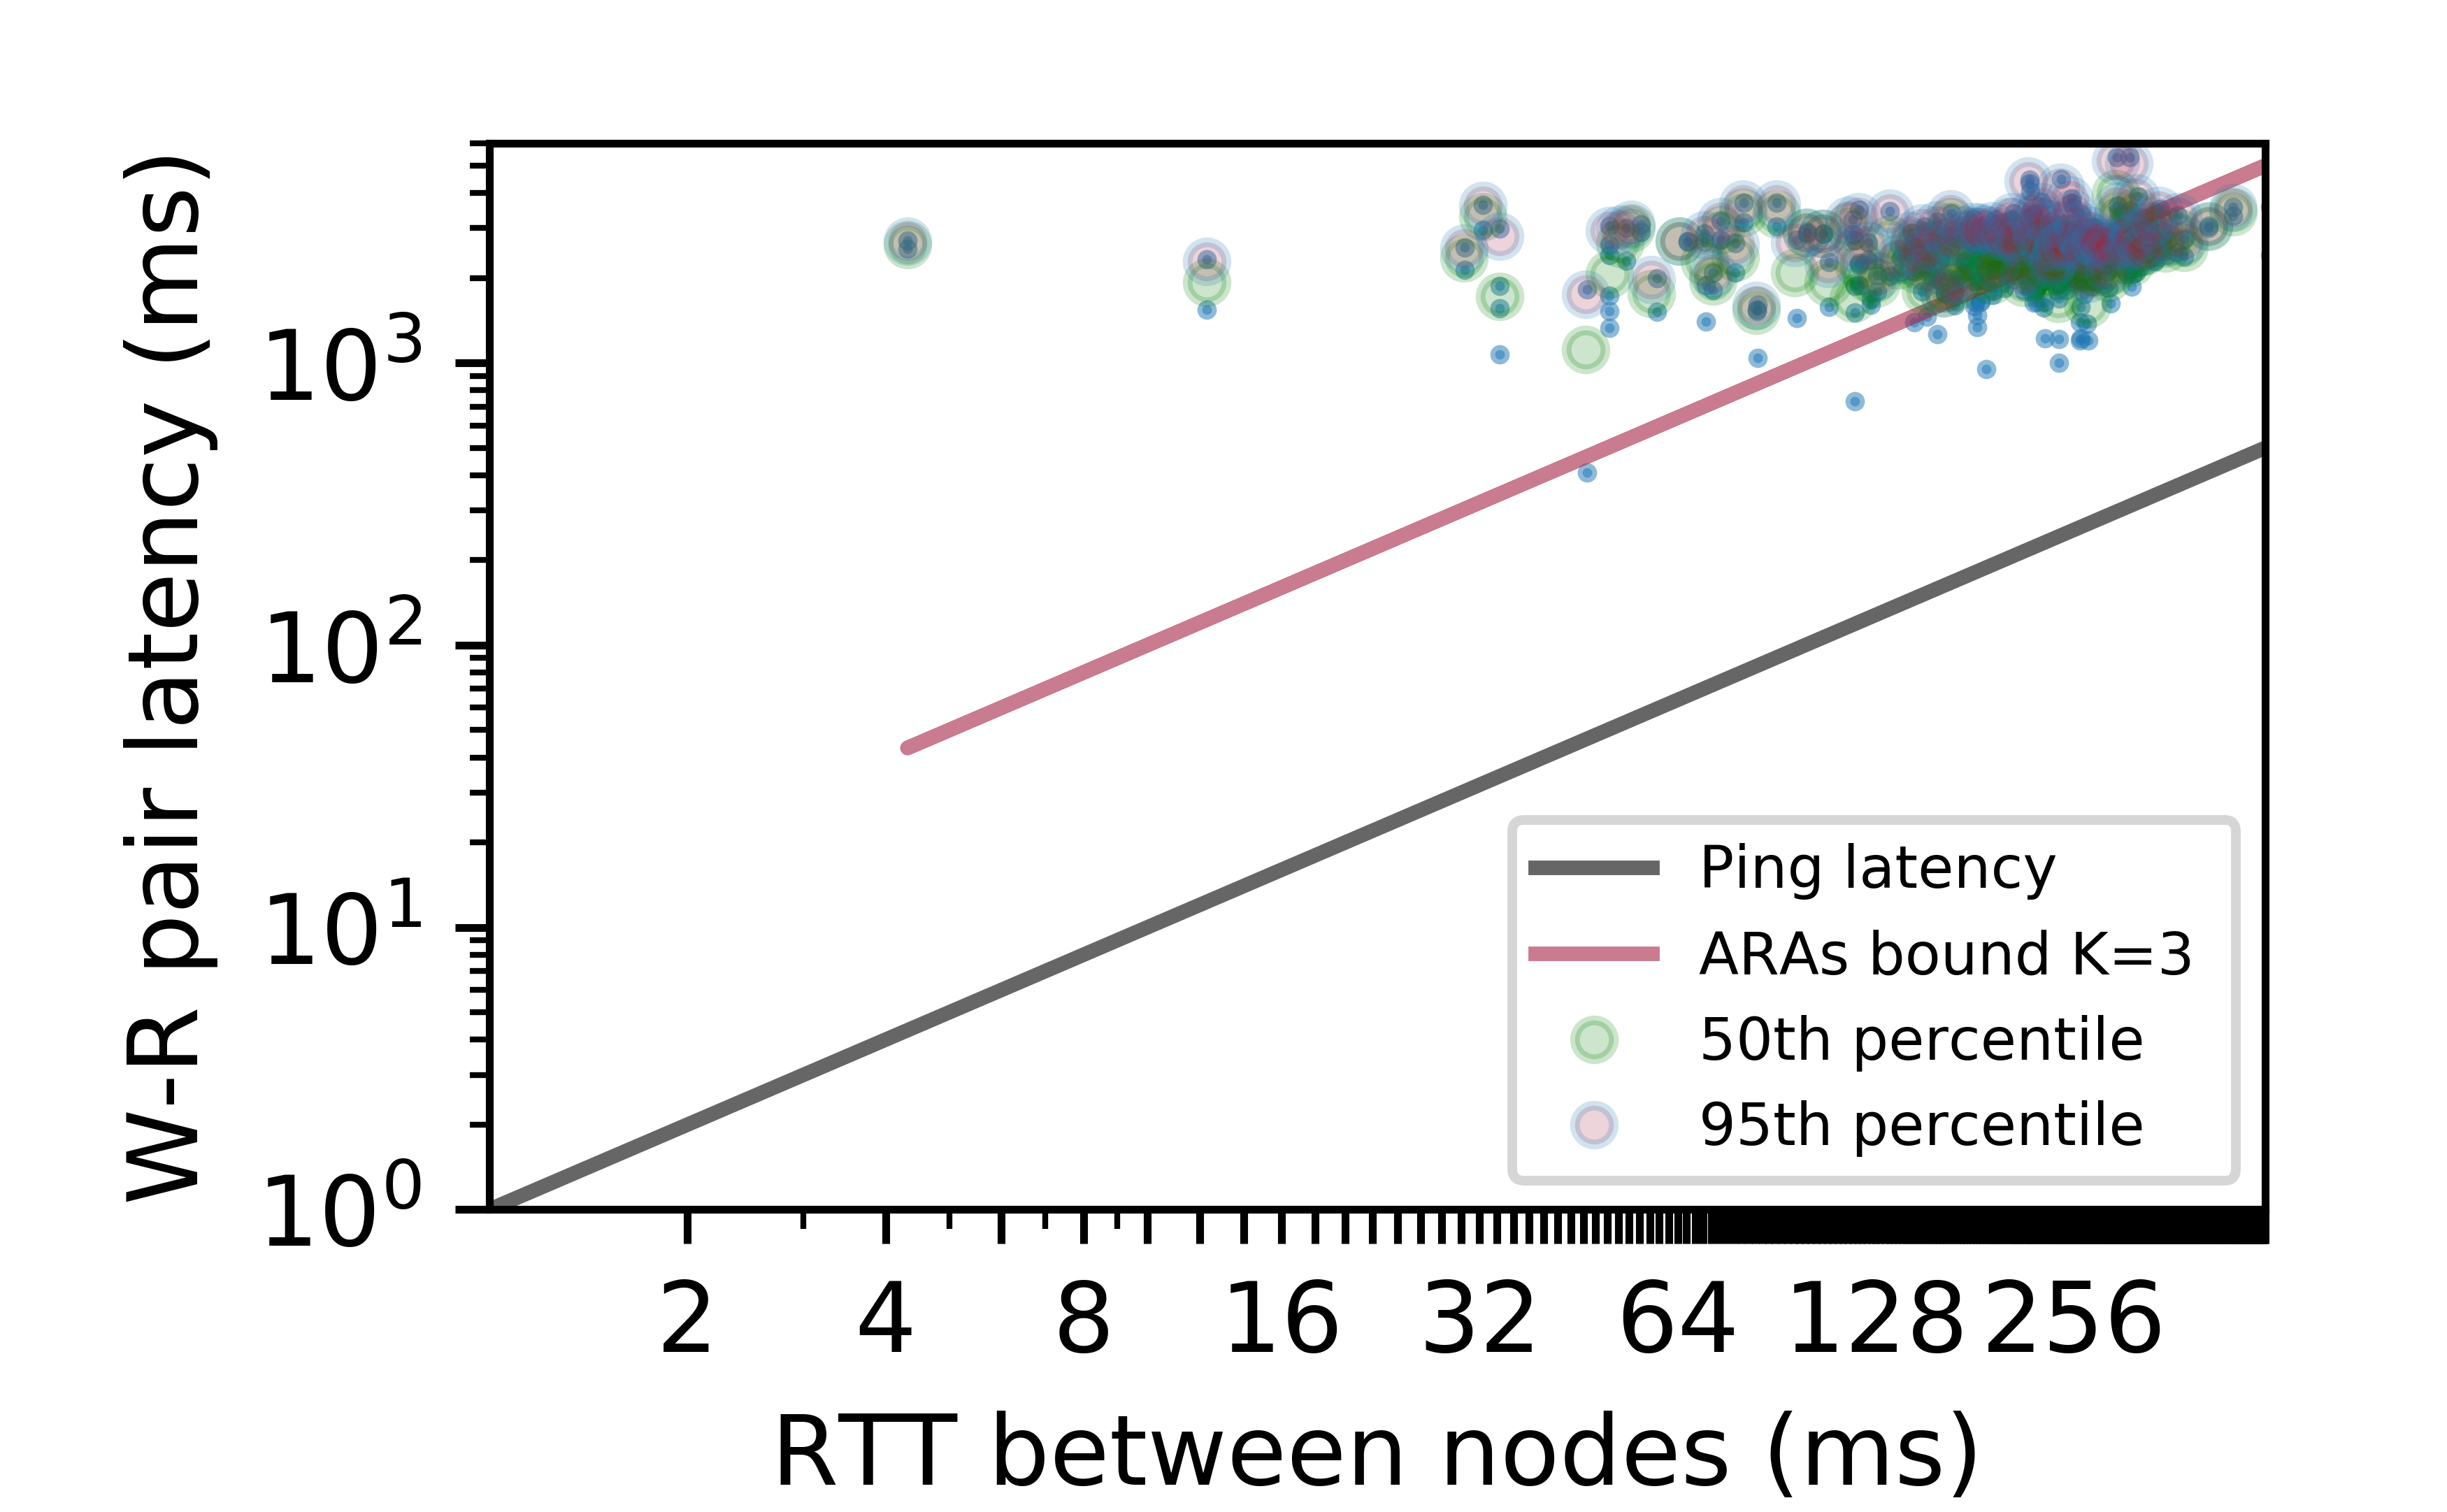
\includegraphics[width=1\linewidth]{graphs/plot_log_vanilla_crdt.png}
  \caption{Vanilla IPFS}
  \label{fig:log1}
\end{subfigure}%
\begin{subfigure}{.5\textwidth}
  \centering
  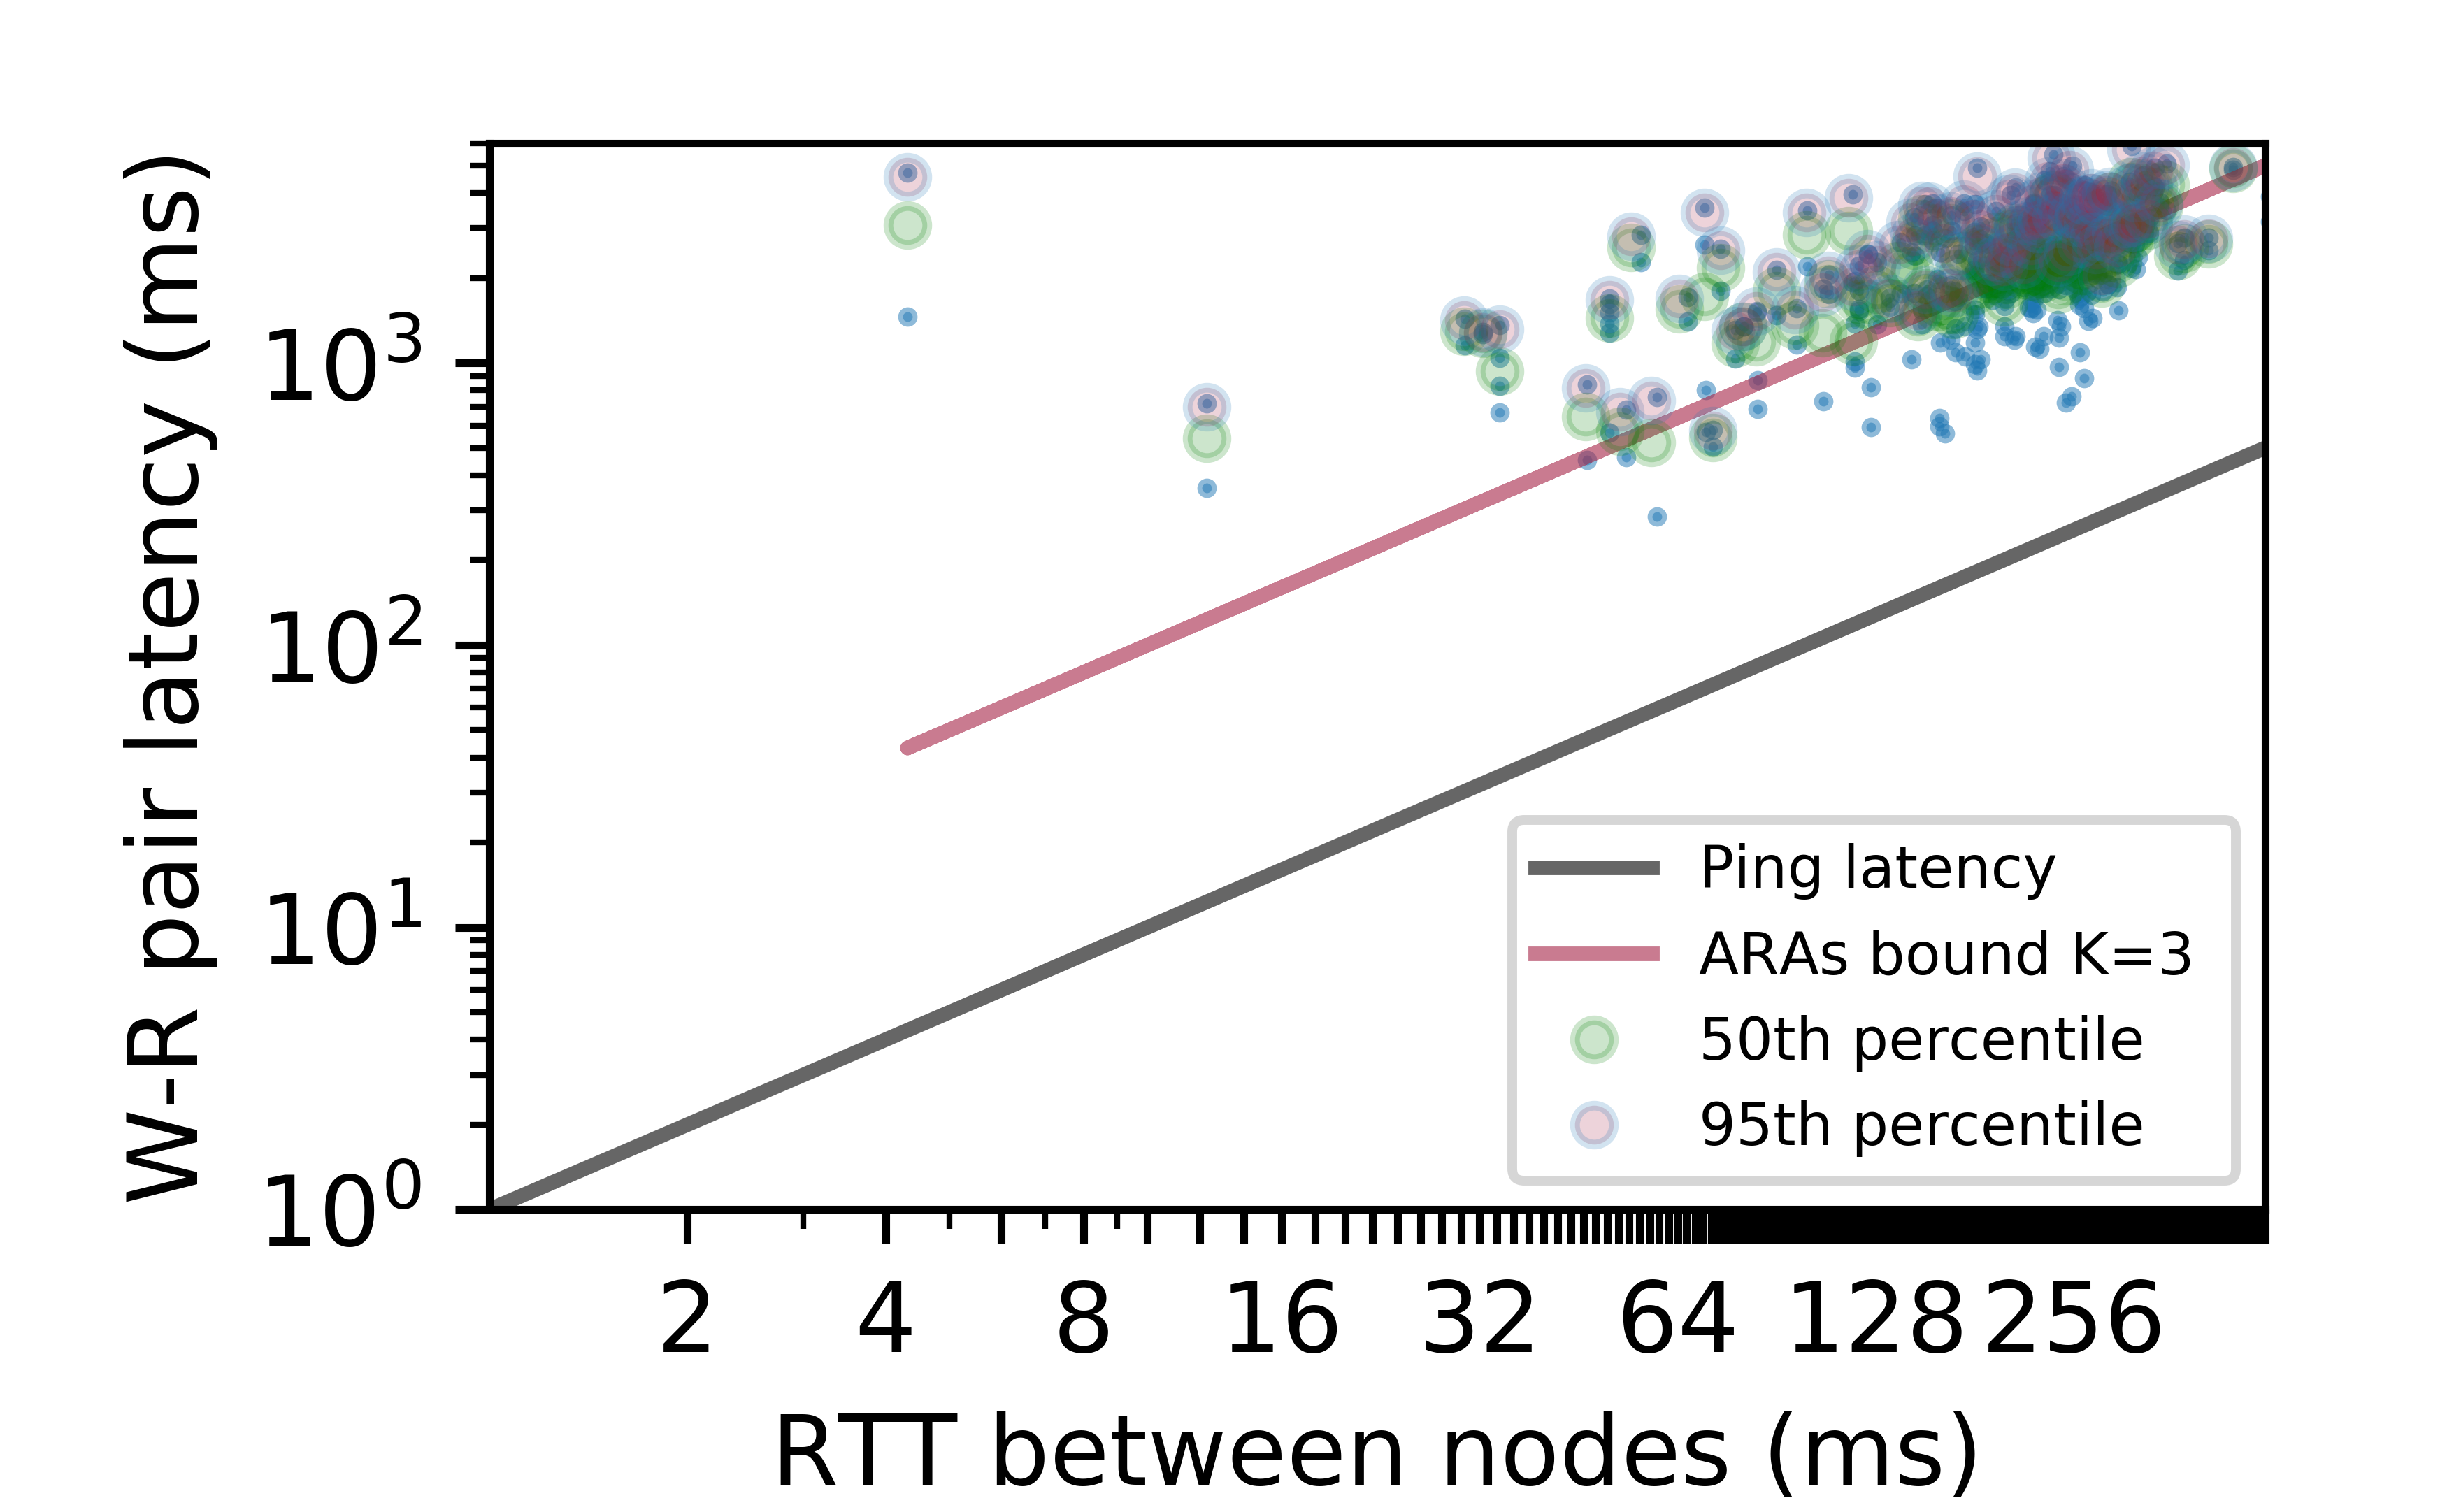
\includegraphics[width=1\linewidth]{graphs/plot_log_cruxified_crdt.png}
  \caption{Cruxified IPFS}
  \label{fig:log2}
\end{subfigure}
\caption{Raft mode, Write+Read latencies}
\label{fig:log}
\end{figure}


\begin{figure}[h!]
  \centering
  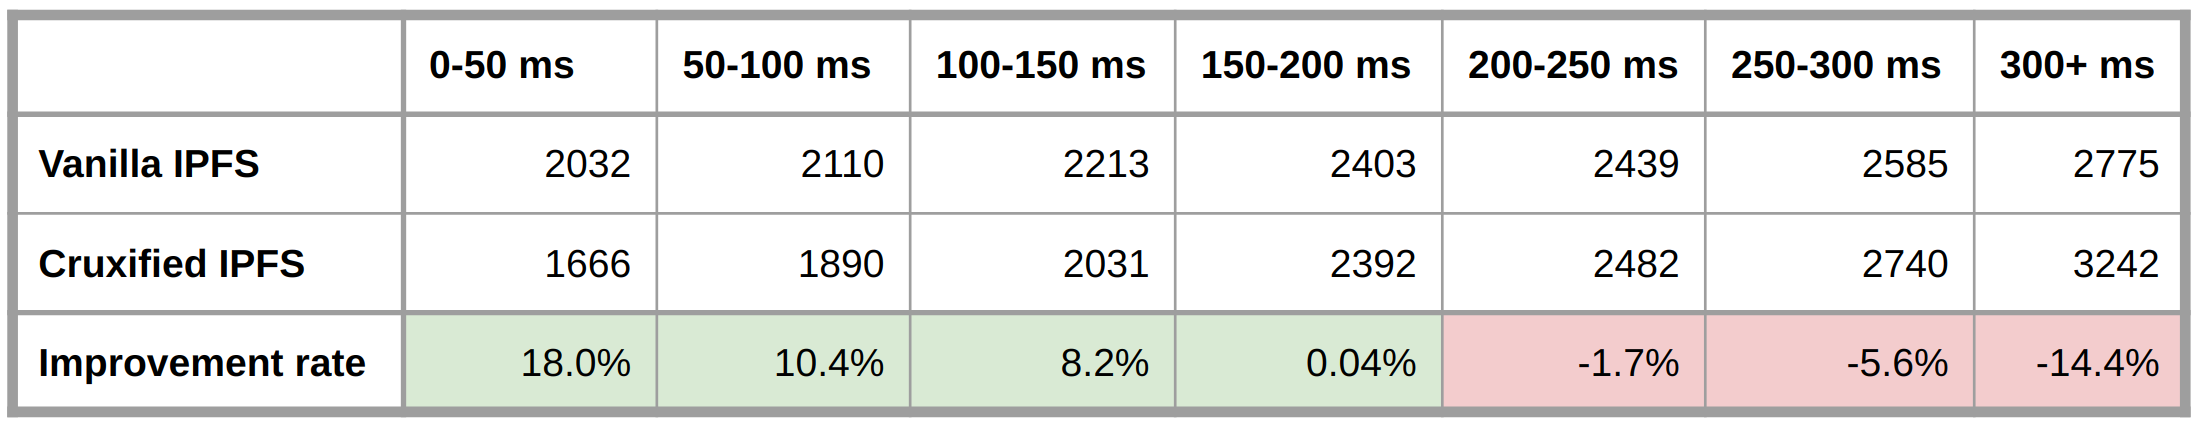
\includegraphics[width=1\linewidth]{tables/writeread.png}
  \caption{Average pair interaction latency according to the RTT between the writer and the reader}
  \label{tab:wr}
\end{figure}

Figures \ref{fig:crdt}, \ref{fig:zoom} and \ref{fig:log} represent the sum of the write and read latency in term of the distance between the writer and the reader nodes. In Cruxified IPFS, we plotted the data from operation performed in the \textit{fastest ARA}. The fastest ARA is defined as the one having the lowest Write+Read latency, hence it is in most cases the ARA with the lowest diameter. This ARA will most likely be the smallest common ARA to the writer and the reader. We selected this metric to show the difference of performance relatively to the RTT between the writer and the reader.

\section{Raft vs CRDT}

We clearly observe on Figures \ref{fig:crdt} and \ref{fig:zoom} that IPFS Cluster has a similar Write+Read latency shape for both consistency components Raft and CRDT, in the Vanilla and Cruxified experiments. Both experiments implement the Crux with Eventual Consistency, thus it made more sense to analyse the results with IPFS Cluster in CRDT mode. Further analysis will be performed with IPFS Cluster in CRDT mode only.

\section{Vanilla vs Cruxified IPFS}

Figure \ref{fig:zoom} and Figure \ref{fig:log} show the performance of respectively vanilla IPFS and cruxified IPFS, with IPFS Cluster in CRDT mode. Figure \ref{fig:log} shows the results at a logarithmic scale, while Figure \ref{fig:zoom} shows the results at a linear scale. 

We can observe in Figure \ref{fig:log} that Cruxified IPFS performance is only slightly better than the vanilla version. But the logarithmic scale is not precise enough for a deeper analysis. This is so because as the distance between the nodes is random, most of the dots will be located close to each other in the logarithmic scale.
Figure \ref{fig:log} is in the exact same format as Figure 3 from Crux paper \cite{crux}, in order to provide a mean of comparison with \textit{Redis} and \textit{CockroachDB} systems. We can see that the performance and improvements of Crux cannot be compared with IPFS, for IPFS is not exactly a data store but a distributed file system. Write and Read operations in IPFS Cluster are more complex than the same operations in Redis or CockroachDB. Vanilla IPFS locality is already optimized by the combination of Kademlia and Coral, whereas vanilla \textit{Redis} and vanilla \textit{CockroachDB} have no locality optimization.

Figure \ref{fig:zoom} is more insightful and shows more precisely that the Write+Read pair latency is lower in Cruxified IPFS than in Vanilla IPFS for low latency pairs of nodes, as expected. Based on Figure \ref{tab:wr}, the average latency improvement on Write+Read operations for pairs of nodes that have a RTT below to 50 ms is $18.0\%$. We can observe that the Write+Read pair latency depends on the RTT between the writer and the reader.
Surprisingly, we observe that Vanilla IPFS performs better than IPFS for high latency pairs of nodes. To understand why Cruxified IPFS is slower than Vanilla IPFS, we will decompose the pair interaction latency in the Read latency, and the Write latency respectively.

\begin{figure}[htbp!]
\centering
\begin{subfigure}{.5\textwidth}
  \centering
  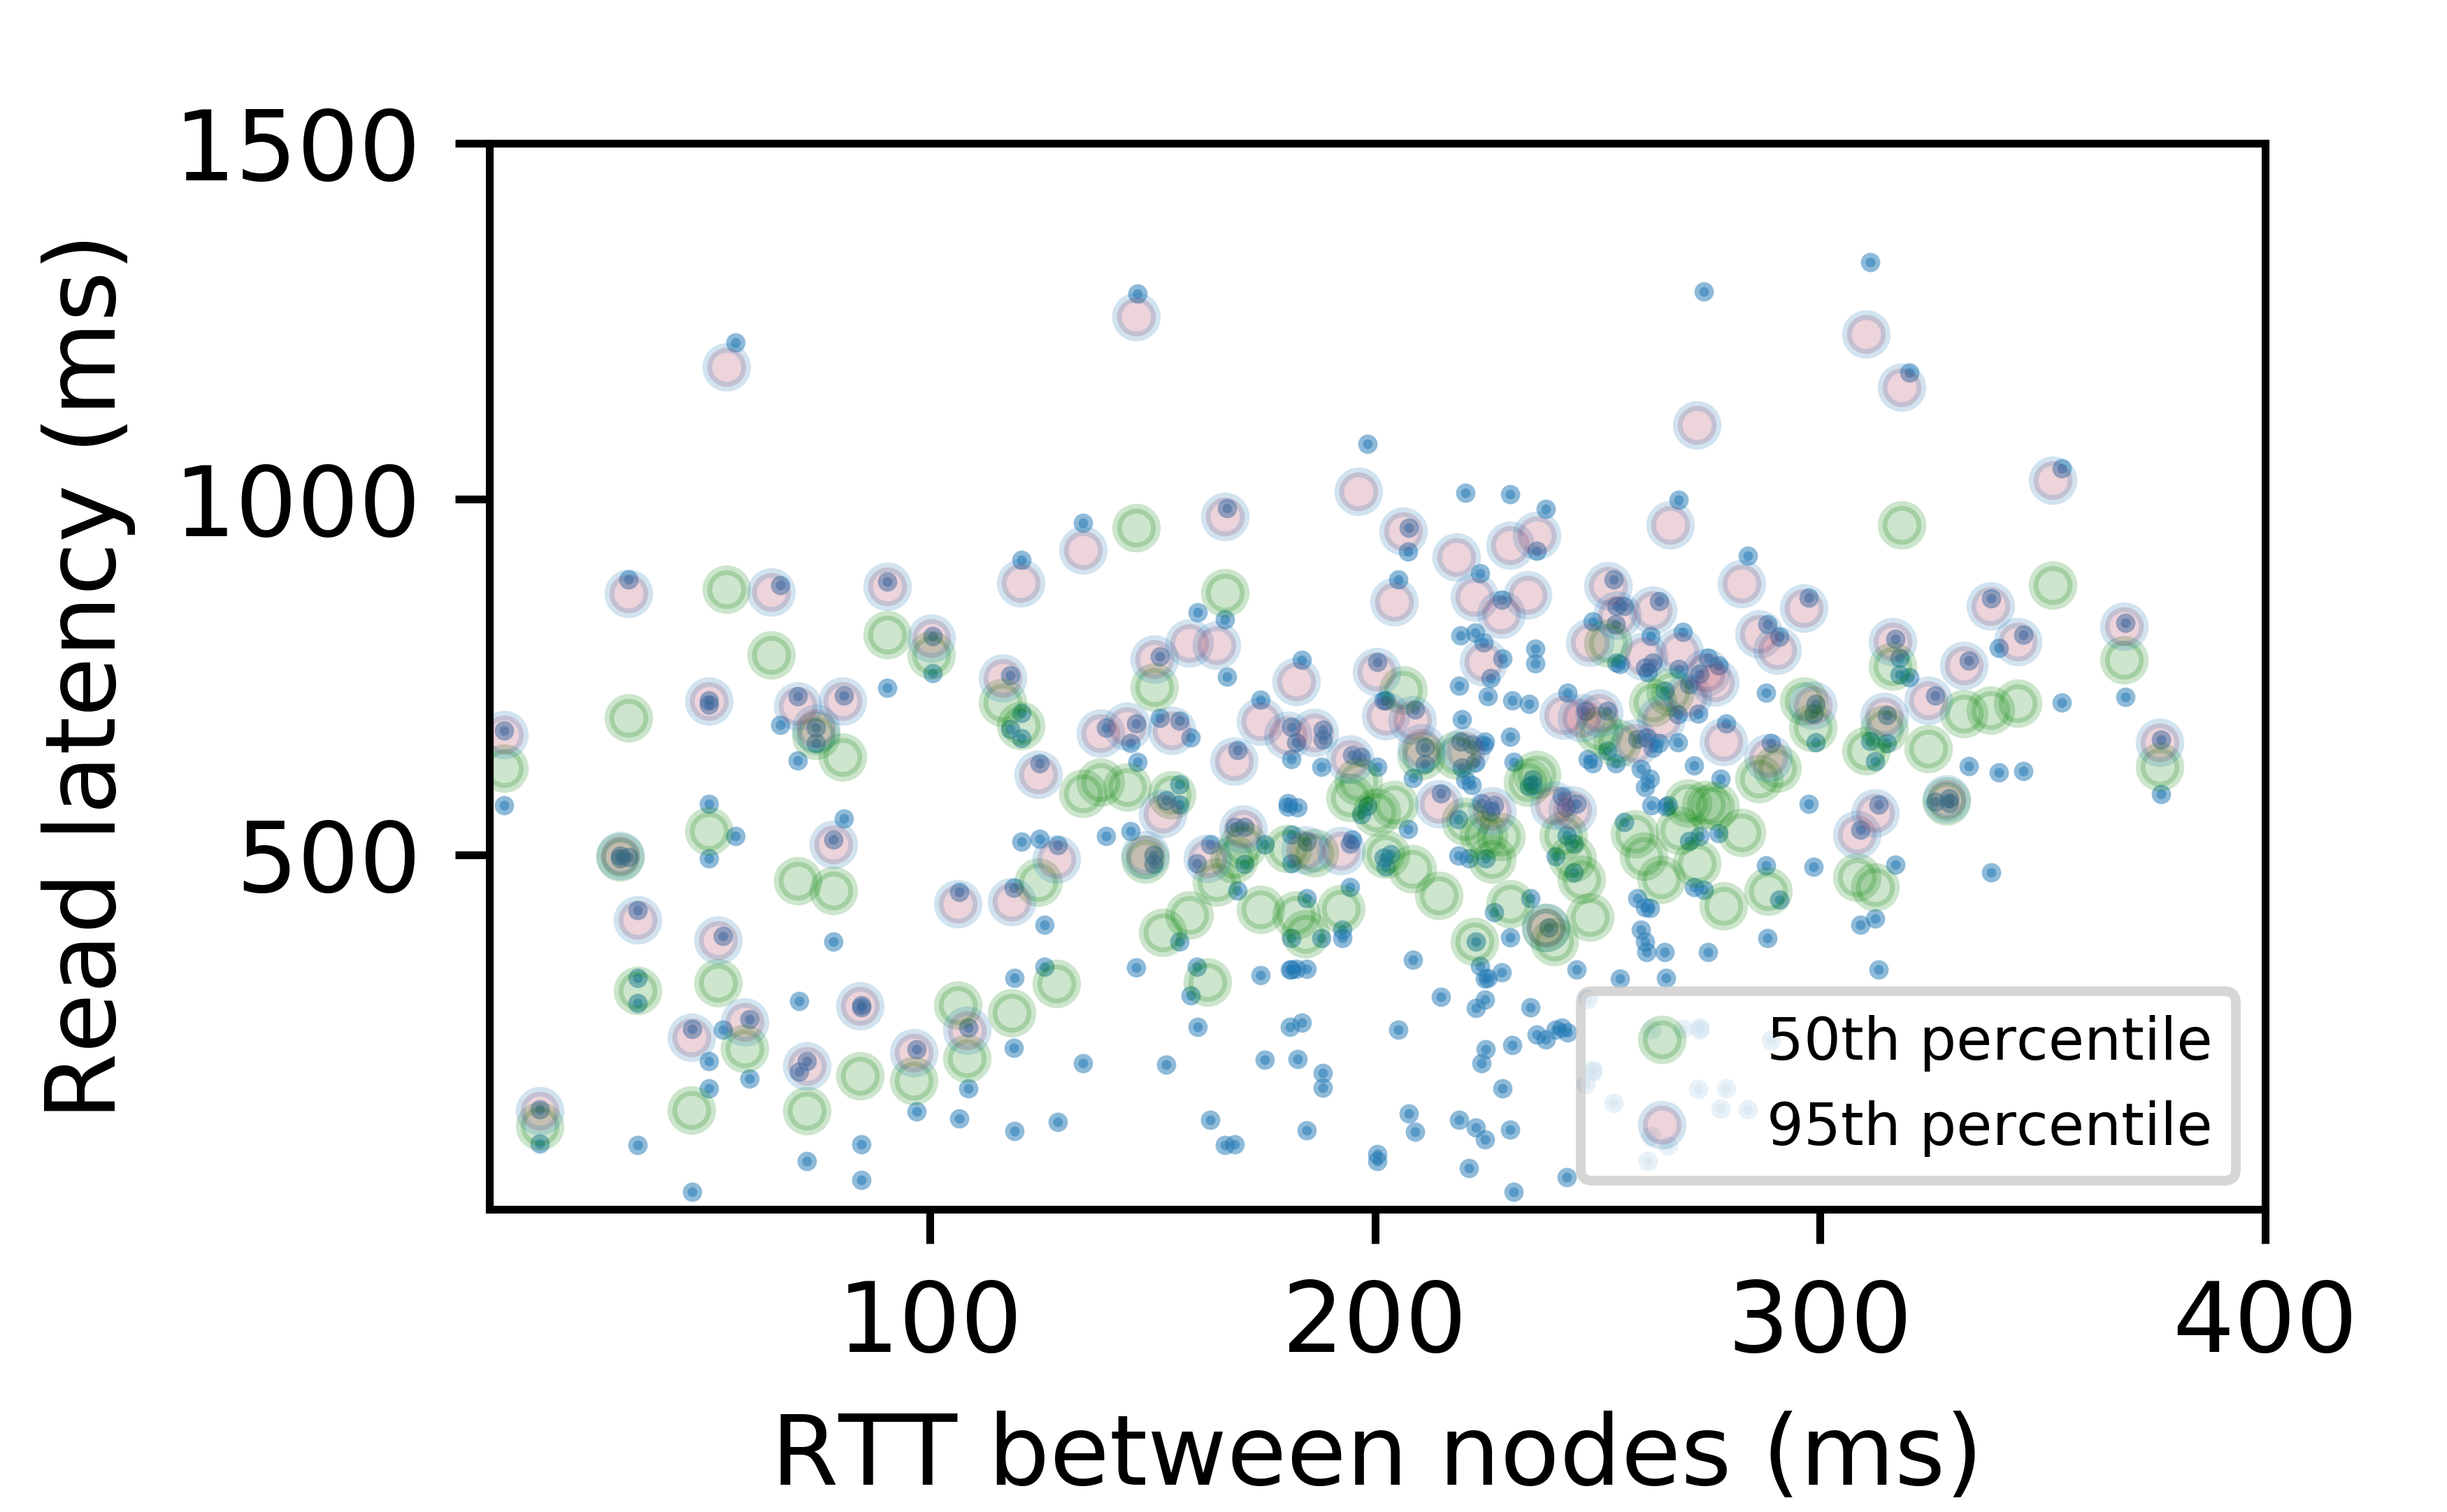
\includegraphics[width=1\linewidth]{graphs/plot_read_vanilla_crdt.png}
  \caption{Vanilla IPFS}
  \label{fig:read1}
\end{subfigure}%
\begin{subfigure}{.5\textwidth}
  \centering
  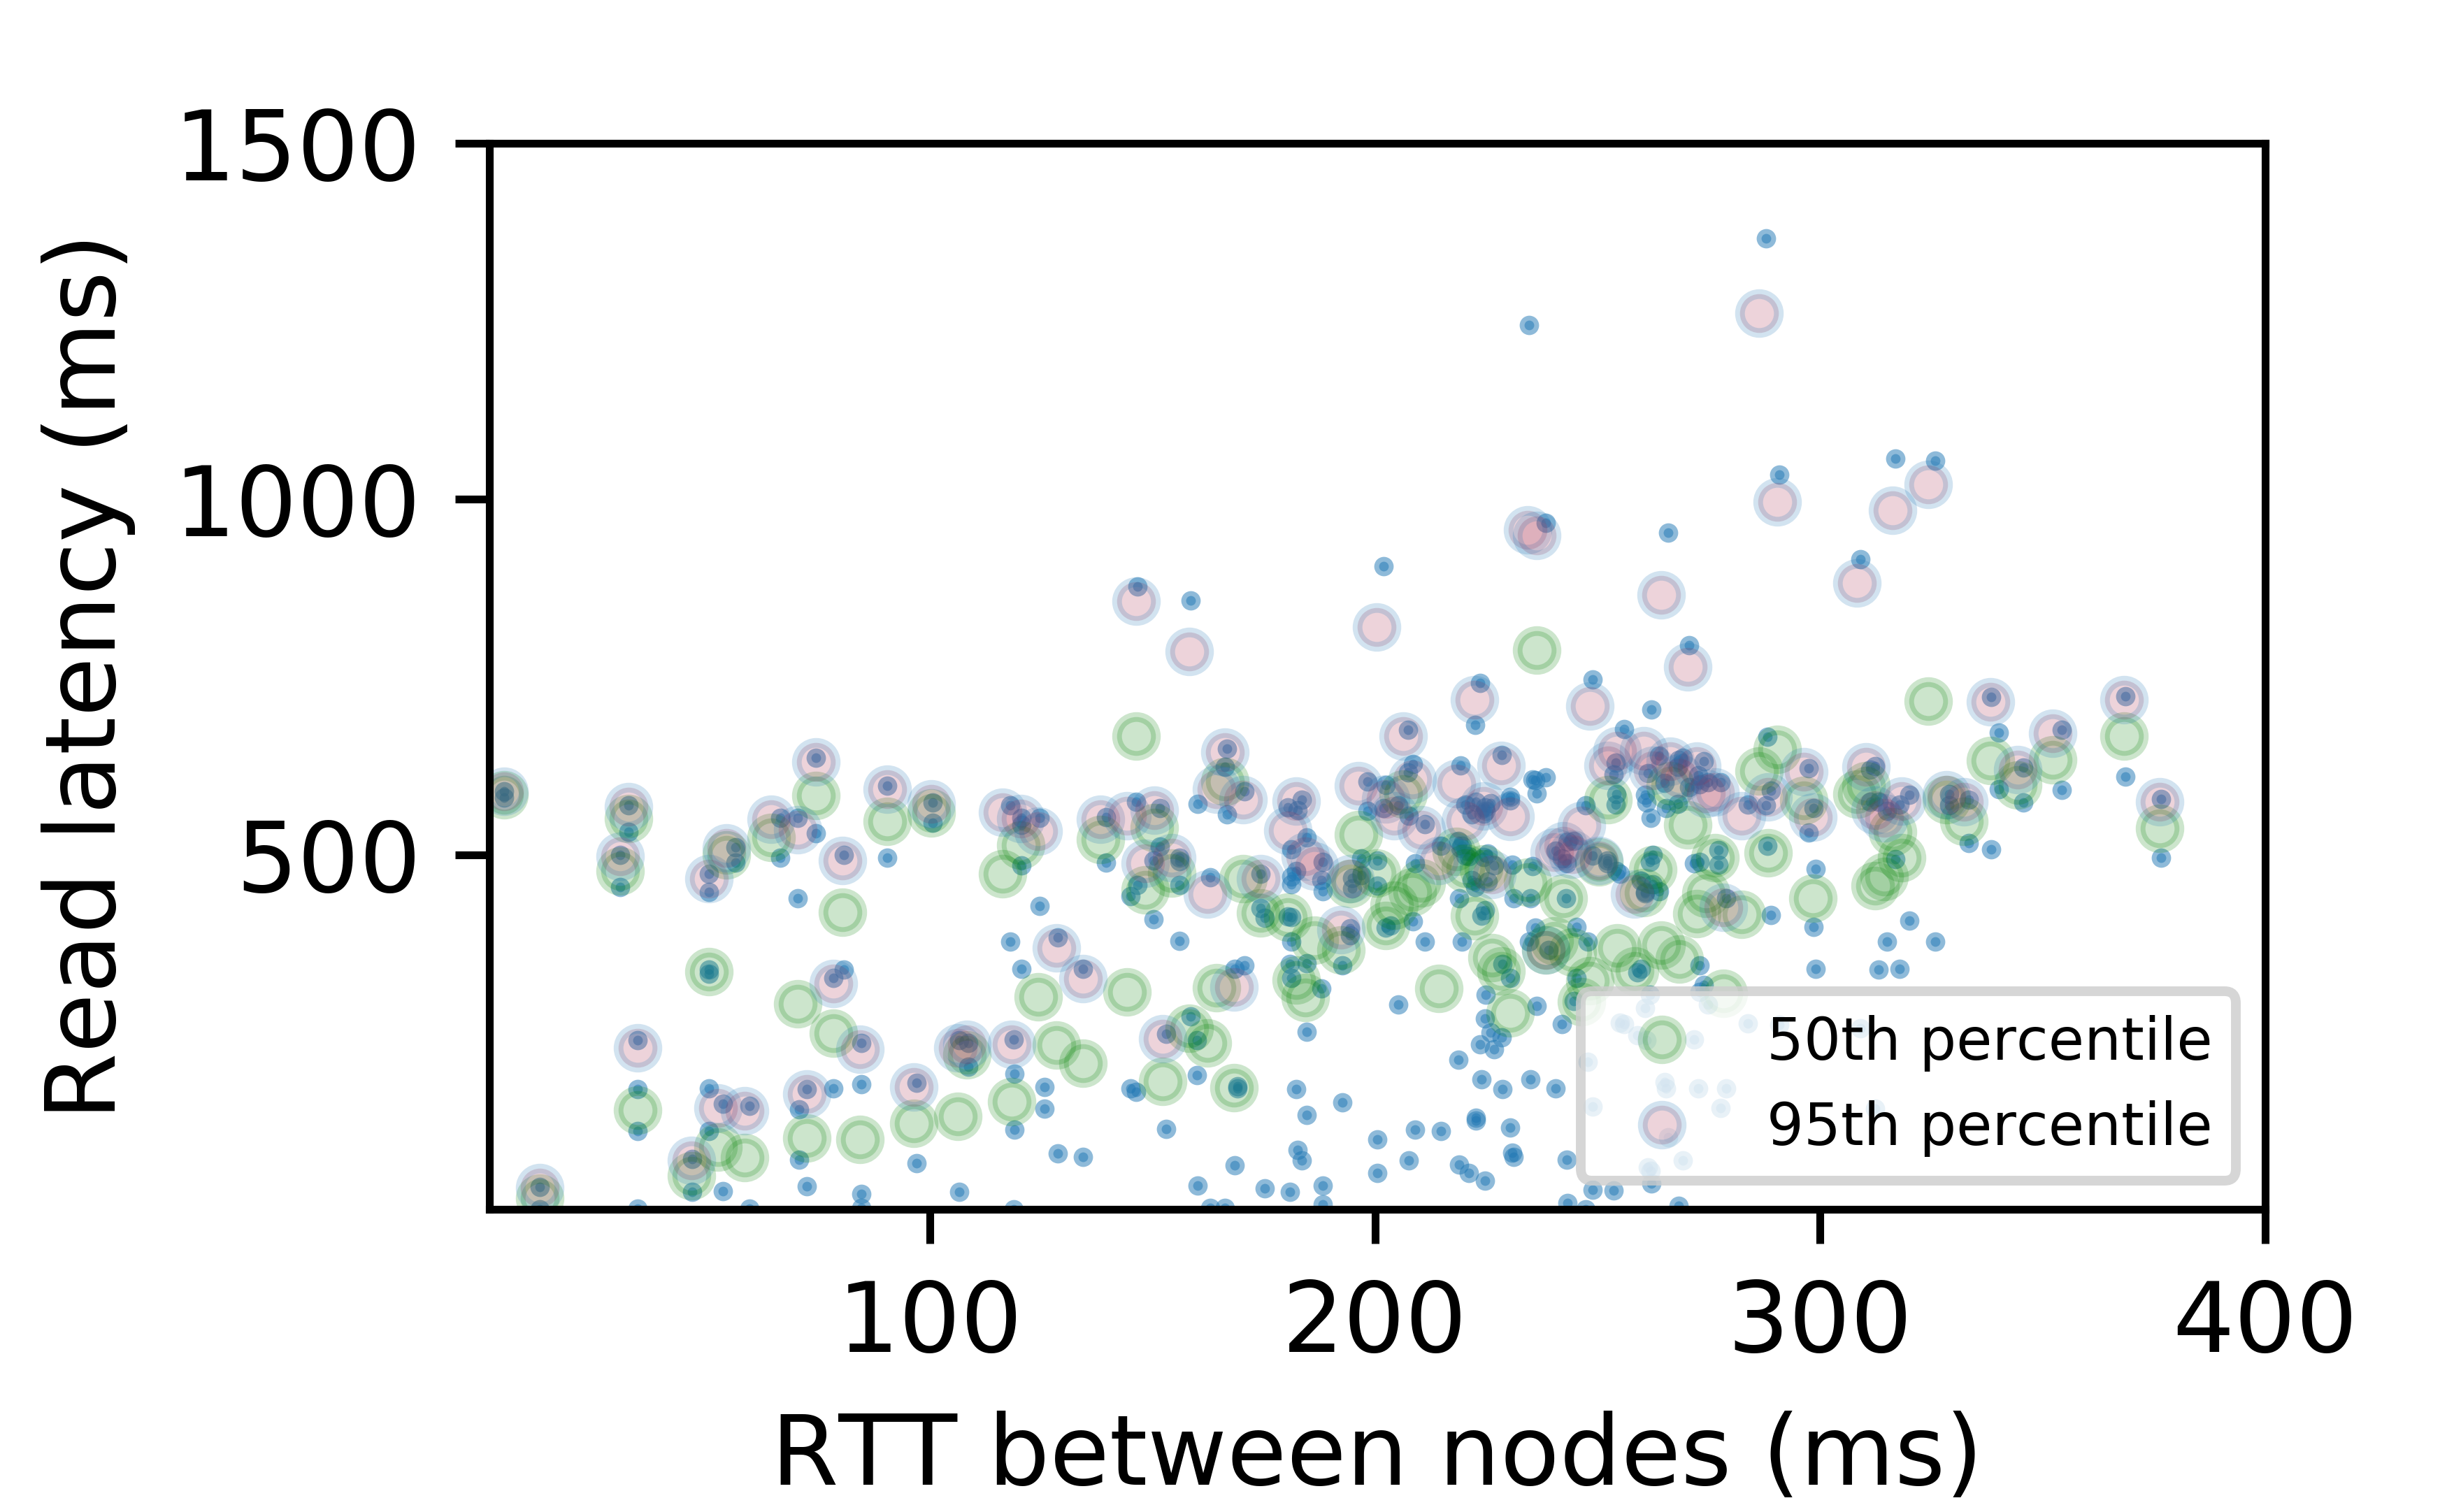
\includegraphics[width=1\linewidth]{graphs/plot_read_cruxified_crdt.png}
  \caption{Cruxified IPFS}
  \label{fig:read2}
\end{subfigure}

\caption{Raft mode, Read latencies}
\label{fig:read}
\end{figure}

\begin{figure}[h!]
  \centering
  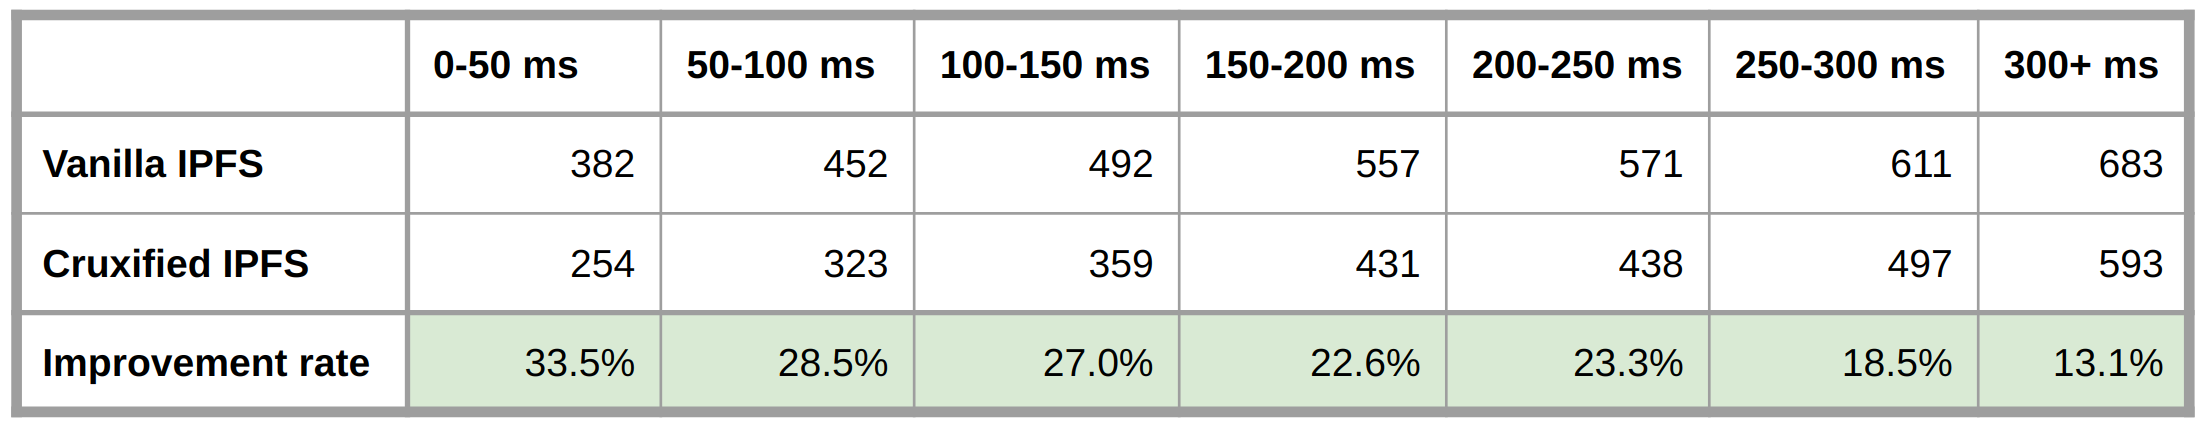
\includegraphics[width=1\linewidth]{tables/read.png}
  \caption{Average pair read latency according to the RTT between the writer and the reader}
  \label{tab:r}
\end{figure}

Figure \ref{fig:read} represents the Read operation latency in terms of the RTT between the writer and reader nodes. Figure \ref{tab:r} shows the average read latency taken from the total pair interaction latency, according to the RTT between the two nodes. Here we observe that Cruxified IPFS always have a lower read lactency compared with Vanilla IPFS. We can see that the the improvement is larger when with low latency pairs of nodes than with high latency pairs of node, which is the expected result. Cruxified IPFS performs better than Vanilla IPFS even with high latency pairs of nodes, for Cruxified IPFS contains more replicas of the file in the global ARA, thus it is likely that one of the replicas will be stored close to the reader on average. The improvement rate that Crux provides to IPFS for the read latency is $13.1\%$ for pairs of nodes with RTT above 300 ms, up to $33.5\%$ for pairs of nodes with RTT below 50 ms.

We also observe that the read latency for Vanilla IPFS increase when the RTT between the reader and the writer increase. This is because 2 RTT are required by IPFS to fetch a file. The IPFS instance first needs to query to DSHT to learn the file location, and then query the file provider. The DSHT storage location is optimized by Coral, as described in the Background section. Thus query latency to the DSHT is optimized in Vanilla IPFS, and Cruxified IPFS optimize the second query latency, to fetch the file from its provider. We notice that the read latency is approximately a fifth of the total pair interaction latency.

\begin{figure}[htbp!]
\centering
\begin{subfigure}{.5\textwidth}
  \centering
  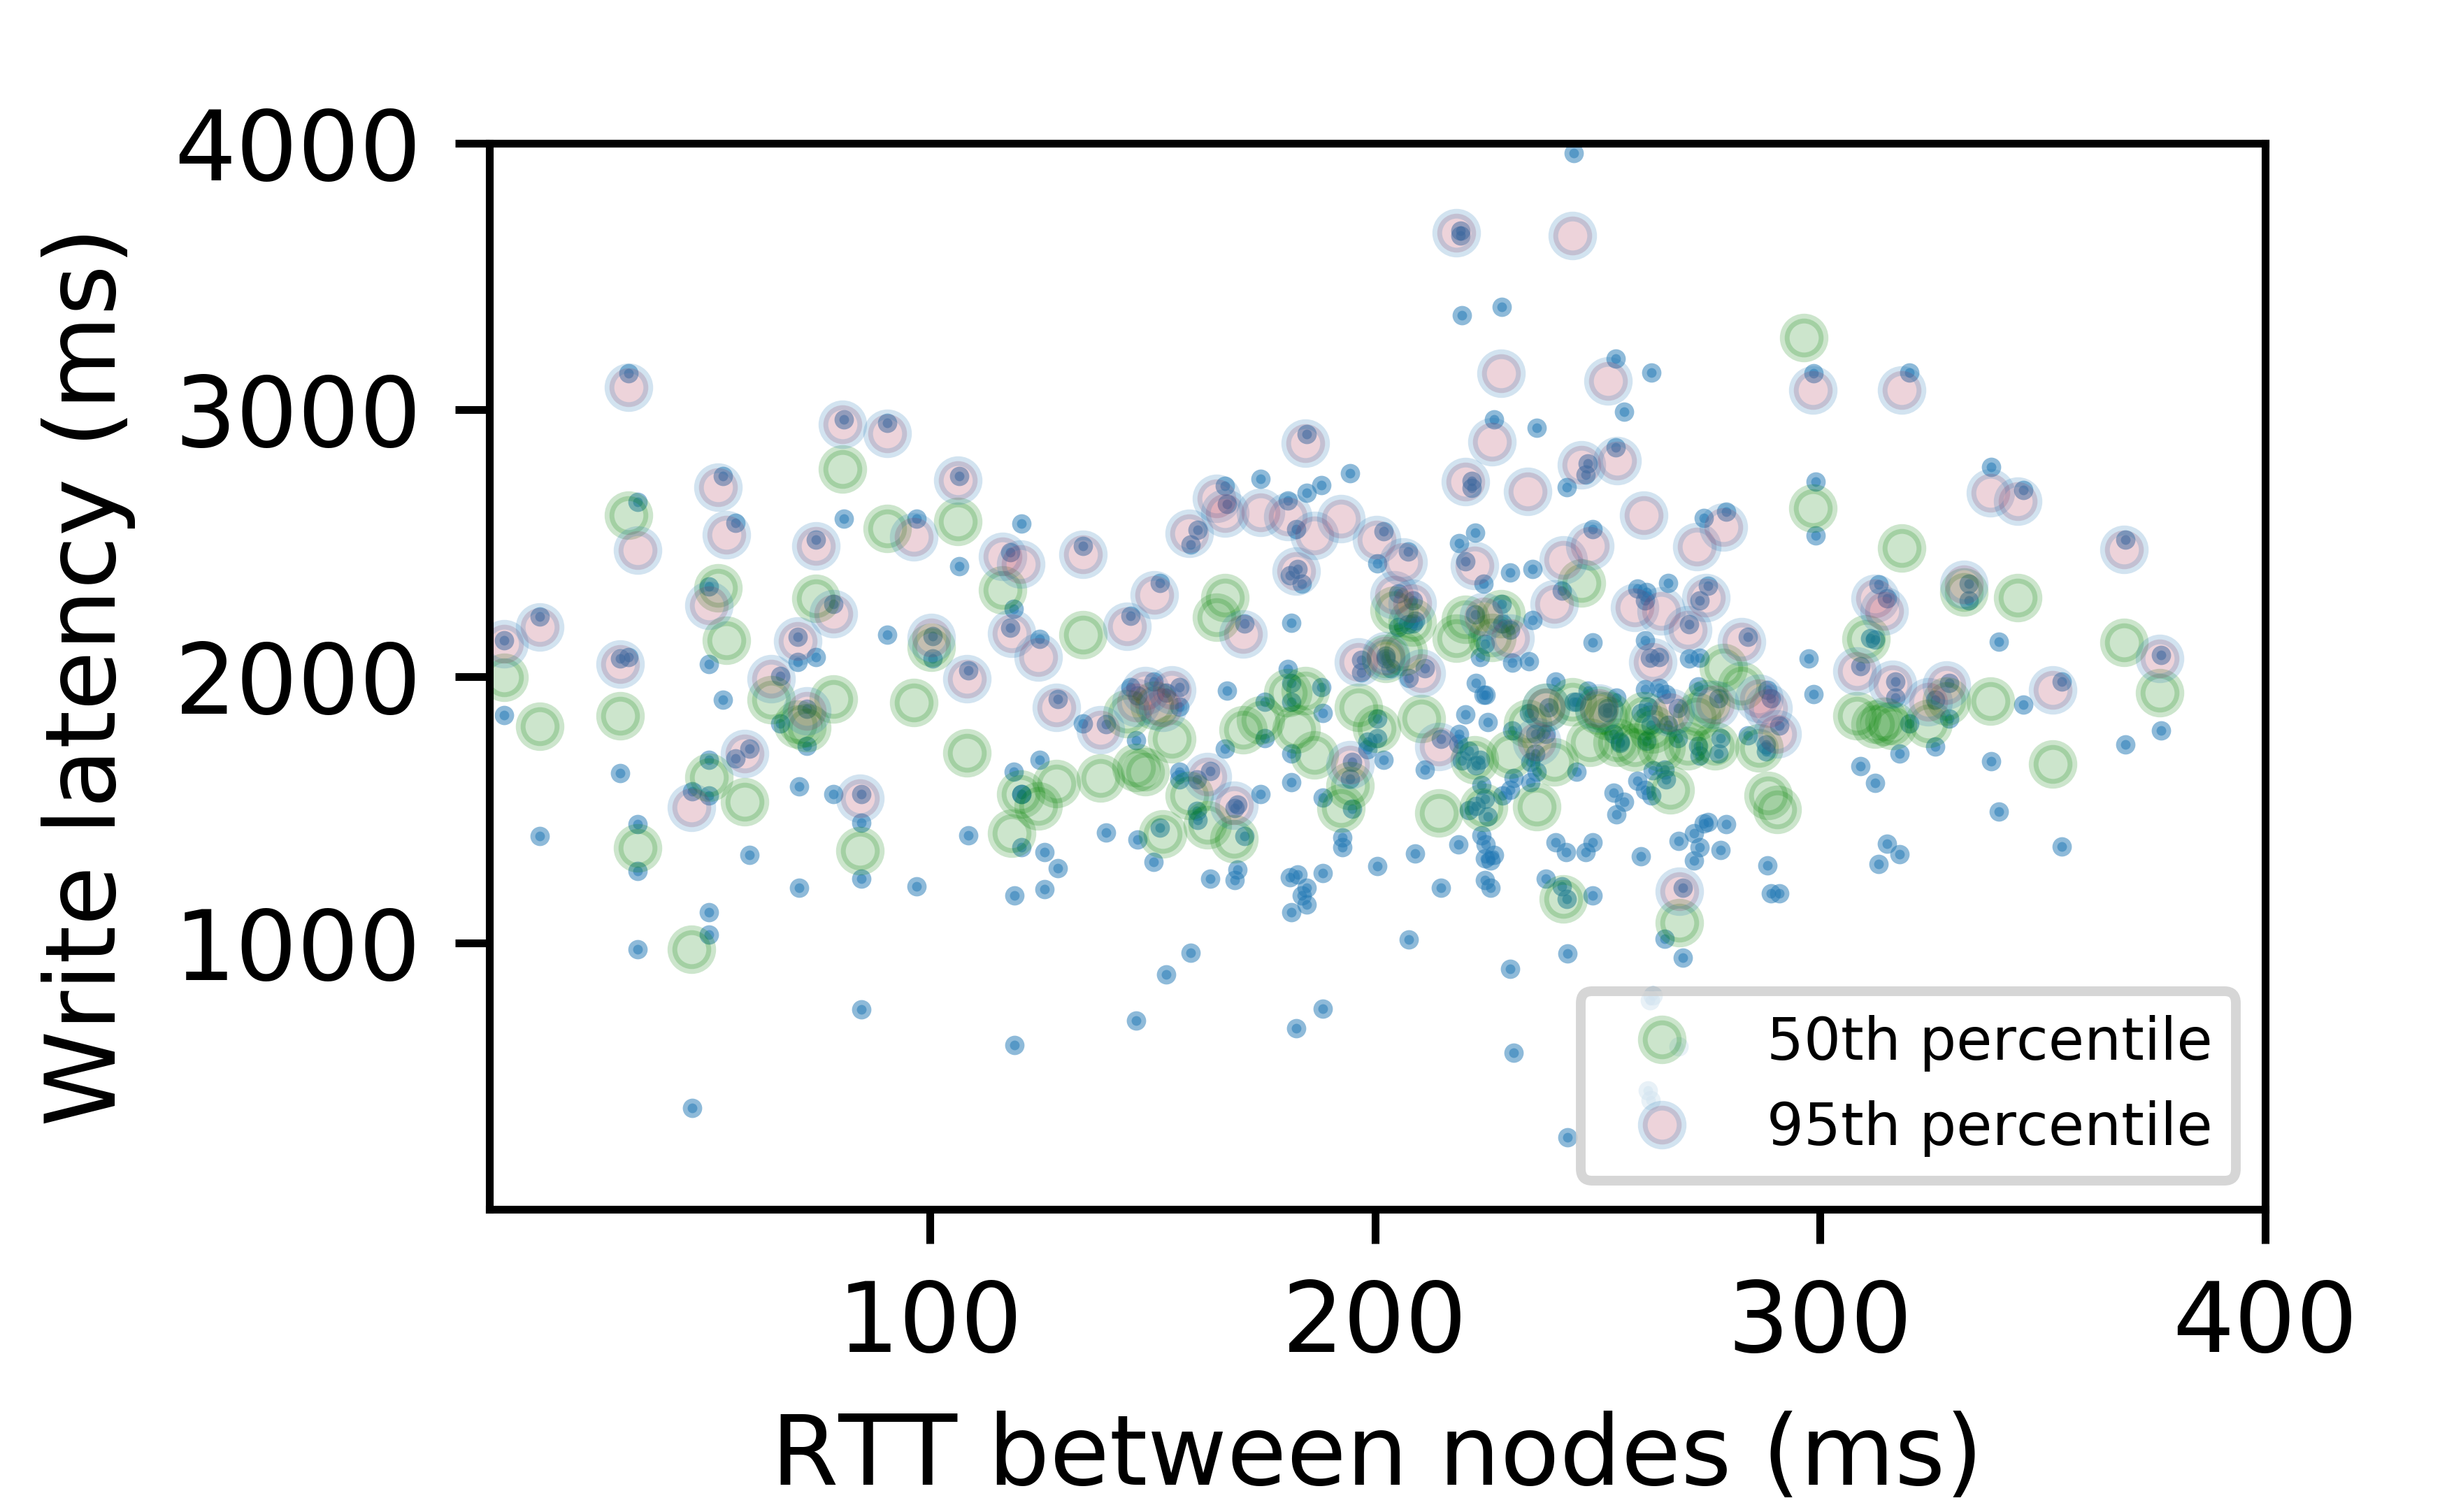
\includegraphics[width=1\linewidth]{graphs/plot_write_vanilla_crdt.png}
  \caption{Vanilla IPFS}
  \label{fig:write1}
\end{subfigure}%
\begin{subfigure}{.5\textwidth}
  \centering
  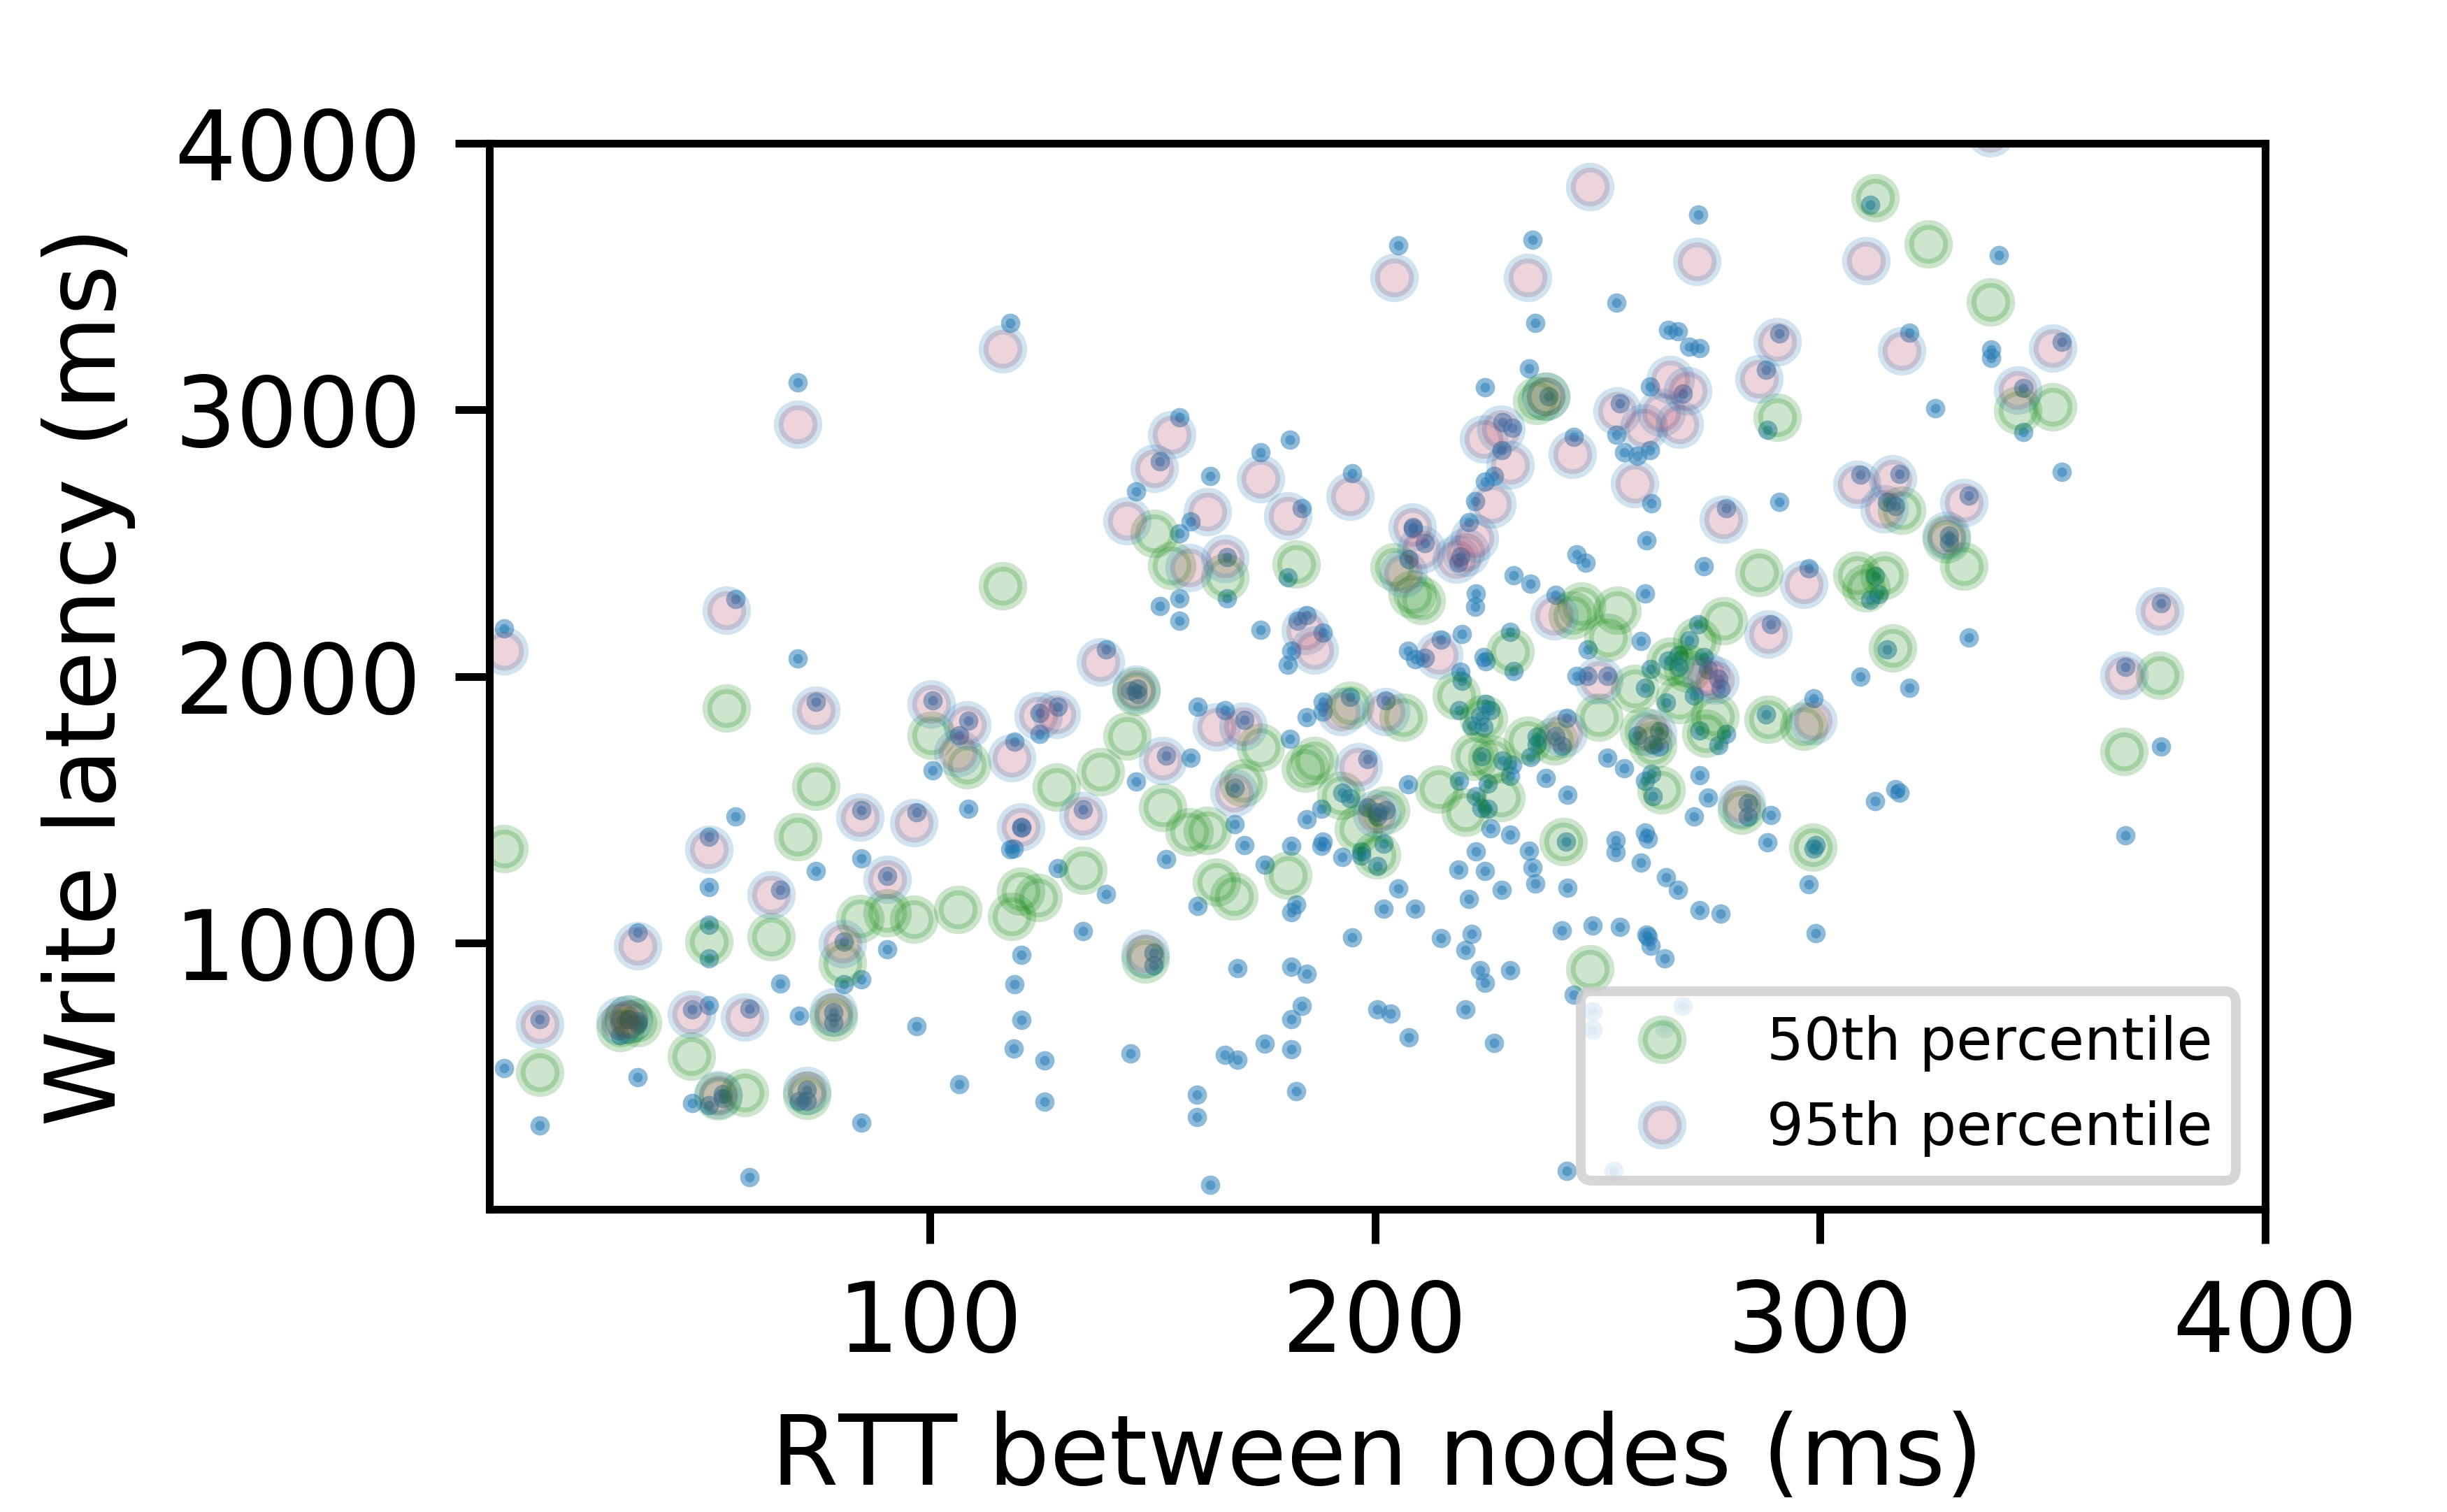
\includegraphics[width=1\linewidth]{graphs/plot_write_cruxified_crdt.png}
  \caption{Cruxified IPFS}
  \label{fig:write2}
\end{subfigure}

\caption{Raft mode, Write latencies}
\label{fig:write}
\end{figure}

\begin{figure}[h!]
  \centering
  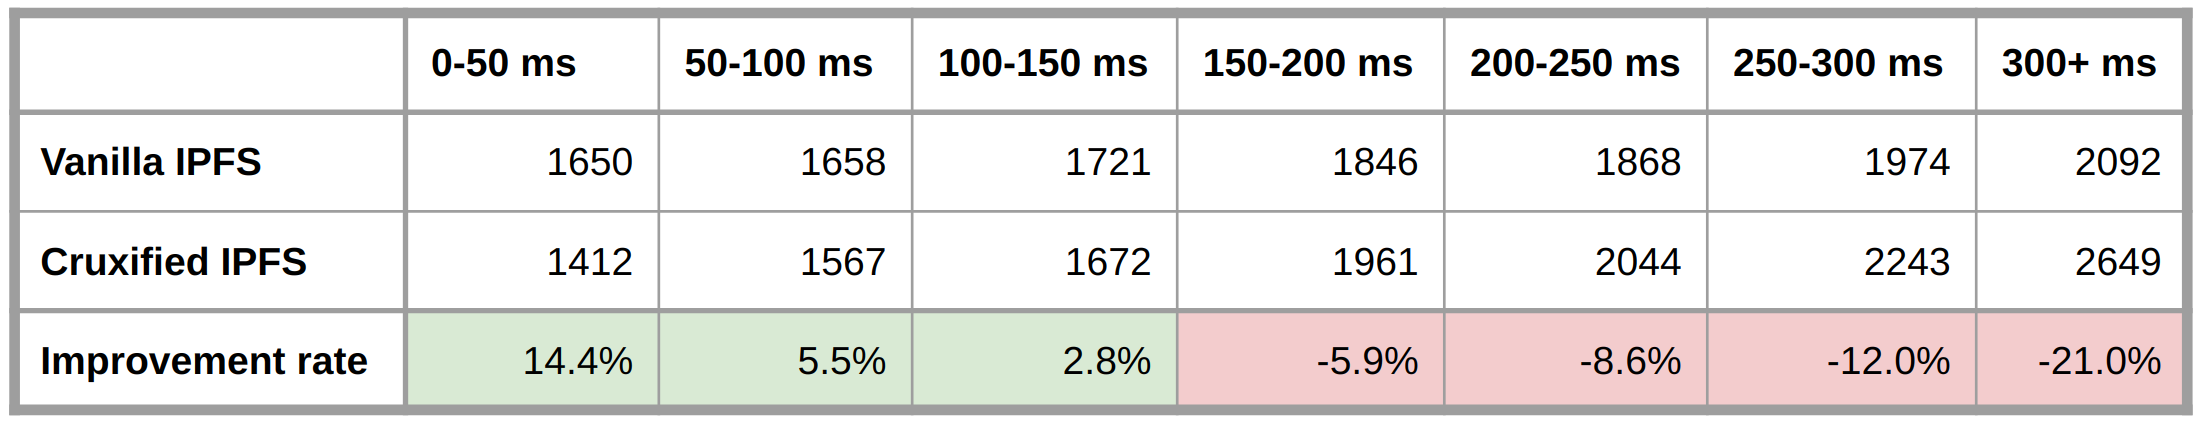
\includegraphics[width=1\linewidth]{tables/write.png}
  \caption{Average pair write latency according to the RTT between the writer and the reader}
  \label{tab:w}
\end{figure}


In Figure \ref{fig:write}, we observe that the write (to the smallest common ARA) latency seems linear in the RTT between the writer and the reader in Cruxified IPFS. From Figure \ref{tab:w} we observe that the write latency depends on the RTT between the writer and the reader, as the write latency is roughly 2x less for pairs of nodes with a RTT lower than 50 ms compared with pairs of nodes with RTT higher than 300 ms. It makes sense, because when the distance between the two nodes is small they will belong to a small common ARA. The time required to reach a consensus in an ARA will be low if nodes are close to each other and if the ARA has a small number of peers. Moreover, in smaller clusters, the file will be allocated to closer nodes, reducing the latency of file transfer to its future providers. Hence, the Write latency will be lower in short diameter clusters, namely small ARAs in Min Cruxified IPFS, than in the global cluster used by Vanilla IPFS, and most likely by Max Cruxified IPFS.


We see that Cruxified IPFS has a lower write latency than Vanilla IPFS for low latency pairs of nodes, but a higher write latency for high latency pairs of nodes. 

When measuring the write latency to the global clusters in Cruxified IPFS, we observed that nodes belonging to many ARAs are slower than nodes belonging to only a few ARAs. As nodes have to run one IPFS daemon and one IPFS Cluster daemon for each cluster membership, nodes belonging to many clusters in Cruxified IPFS are slowed down. Both daemons are greedy in RAM, and thus the 16GiB RAM are not enough to run all the daemons at full speed. As Vanilla IPFS only runs a single instance of IPFS and a single instance of IPFS Cluster, it will on average be faster than any node in the Cruxified IPFS to write to a global ARA. Thus, this explains why Vanilla IPFS has a lower write latency for pairs of nodes with high latency, interacting through large diameter ARAs. If IPFS Cluster provided a way to manage multiple clusters on the same instance, without any RAM overhead, we would have a better performance for Cruxified IPFS.

Overall, we get a slight improvement, of on average $18.0\%$ on the Write+Read pair latency for pairs of nodes with the latency between the writer and the reader below 50 ms, for the system in an eventually consistency setting. We observed that the performance of Cruxified IPFS is not as good as we expected because the hosts are slowed down by too many IPFS and IPFS Cluster daemons. The observed improvement comes at the cost of a storage overhead. This overhead was not measured in this experiment, but according to Crux \cite{crux}, it is logarithmic in terms of the network size.


%%%%%%%%%%%%%%%%%%%%
\chapter{Conclusion}
%%%%%%%%%%%%%%%%%%%%

We showed that Cruxified IPFS has a lower pair interaction latency for low RTT pairs of nodes, than for high latency pairs of nodes. Cruxified IPFS demonstrated on average a lower pair interaction latency than Vanilla IPFS for low latency pairs of nodes. Although, Vanilla IPFS proved to have a lower pair interaction latency than Cruxified IPFS on high latency pairs of nodes. This is so, mainly because the hosts in Cruxified IPFS are running too many IPFS and IPFS Cluster daemons, which slows down all the write operations. If IPFS Cluster handled multiple clusters memberships more efficiently, we would get a lower pair interaction latency for all pairs of nodes. Our experiments, run on a relatively limited network of 20 nodes, demonstrated that interaction latency in Cruxified IPFS in CRDT mode can be up to $18.0\%$ faster than in Vanilla IPFS for a writer and a reader less than 50 ms apart. 
We also observe that the pair interaction latency in IPFS also depends on the latency distance between the writer and the reader. This is so because IPFS DSHT inspired by Coral contains locality optimization, but the file storage location in IPFS Cluster is not optimized. If a single IPFS Cluster instance could handle multiple clusters membership without performance loss, interaction latency in Cruxified IPFS would be faster for all pairs of nodes.

For future work, it would be interesting to reproduce the same experiment on a larger network, composed of thousands of nodes all around the globe to get a better idea of a deployment at a larger scale. Another scaling direction would be to simulate a realistic inter planetary node topology, with a RTT of multiple minutes between some nodes, in order to test Crux in an inter planetary setting. Now that Cruxified IPFS is implemented, we could also test its partition resistance, which is the second locality enhancement defined in Crux.

\addcontentsline{toc}{chapter}{Bibliography}
\printbibliography

\end{document}